% Options for packages loaded elsewhere
\PassOptionsToPackage{unicode}{hyperref}
\PassOptionsToPackage{hyphens}{url}
\PassOptionsToPackage{dvipsnames,svgnames,x11names}{xcolor}
%
\documentclass[
  12pt,
  letterpaper,
]{book}

\usepackage{amsmath,amssymb}
\usepackage{iftex}
\ifPDFTeX
  \usepackage[T1]{fontenc}
  \usepackage[utf8]{inputenc}
  \usepackage{textcomp} % provide euro and other symbols
\else % if luatex or xetex
  \usepackage{unicode-math}
  \defaultfontfeatures{Scale=MatchLowercase}
  \defaultfontfeatures[\rmfamily]{Ligatures=TeX,Scale=1}
\fi
\usepackage{lmodern}
\ifPDFTeX\else  
    % xetex/luatex font selection
\fi
% Use upquote if available, for straight quotes in verbatim environments
\IfFileExists{upquote.sty}{\usepackage{upquote}}{}
\IfFileExists{microtype.sty}{% use microtype if available
  \usepackage[]{microtype}
  \UseMicrotypeSet[protrusion]{basicmath} % disable protrusion for tt fonts
}{}
\makeatletter
\@ifundefined{KOMAClassName}{% if non-KOMA class
  \IfFileExists{parskip.sty}{%
    \usepackage{parskip}
  }{% else
    \setlength{\parindent}{0pt}
    \setlength{\parskip}{6pt plus 2pt minus 1pt}}
}{% if KOMA class
  \KOMAoptions{parskip=half}}
\makeatother
\usepackage{xcolor}
\usepackage[margin=1in]{geometry}
\setlength{\emergencystretch}{3em} % prevent overfull lines
\setcounter{secnumdepth}{5}
% Make \paragraph and \subparagraph free-standing
\makeatletter
\ifx\paragraph\undefined\else
  \let\oldparagraph\paragraph
  \renewcommand{\paragraph}{
    \@ifstar
      \xxxParagraphStar
      \xxxParagraphNoStar
  }
  \newcommand{\xxxParagraphStar}[1]{\oldparagraph*{#1}\mbox{}}
  \newcommand{\xxxParagraphNoStar}[1]{\oldparagraph{#1}\mbox{}}
\fi
\ifx\subparagraph\undefined\else
  \let\oldsubparagraph\subparagraph
  \renewcommand{\subparagraph}{
    \@ifstar
      \xxxSubParagraphStar
      \xxxSubParagraphNoStar
  }
  \newcommand{\xxxSubParagraphStar}[1]{\oldsubparagraph*{#1}\mbox{}}
  \newcommand{\xxxSubParagraphNoStar}[1]{\oldsubparagraph{#1}\mbox{}}
\fi
\makeatother

\usepackage{color}
\usepackage{fancyvrb}
\newcommand{\VerbBar}{|}
\newcommand{\VERB}{\Verb[commandchars=\\\{\}]}
\DefineVerbatimEnvironment{Highlighting}{Verbatim}{commandchars=\\\{\}}
% Add ',fontsize=\small' for more characters per line
\usepackage{framed}
\definecolor{shadecolor}{RGB}{241,243,245}
\newenvironment{Shaded}{\begin{snugshade}}{\end{snugshade}}
\newcommand{\AlertTok}[1]{\textcolor[rgb]{0.68,0.00,0.00}{#1}}
\newcommand{\AnnotationTok}[1]{\textcolor[rgb]{0.37,0.37,0.37}{#1}}
\newcommand{\AttributeTok}[1]{\textcolor[rgb]{0.40,0.45,0.13}{#1}}
\newcommand{\BaseNTok}[1]{\textcolor[rgb]{0.68,0.00,0.00}{#1}}
\newcommand{\BuiltInTok}[1]{\textcolor[rgb]{0.00,0.23,0.31}{#1}}
\newcommand{\CharTok}[1]{\textcolor[rgb]{0.13,0.47,0.30}{#1}}
\newcommand{\CommentTok}[1]{\textcolor[rgb]{0.37,0.37,0.37}{#1}}
\newcommand{\CommentVarTok}[1]{\textcolor[rgb]{0.37,0.37,0.37}{\textit{#1}}}
\newcommand{\ConstantTok}[1]{\textcolor[rgb]{0.56,0.35,0.01}{#1}}
\newcommand{\ControlFlowTok}[1]{\textcolor[rgb]{0.00,0.23,0.31}{\textbf{#1}}}
\newcommand{\DataTypeTok}[1]{\textcolor[rgb]{0.68,0.00,0.00}{#1}}
\newcommand{\DecValTok}[1]{\textcolor[rgb]{0.68,0.00,0.00}{#1}}
\newcommand{\DocumentationTok}[1]{\textcolor[rgb]{0.37,0.37,0.37}{\textit{#1}}}
\newcommand{\ErrorTok}[1]{\textcolor[rgb]{0.68,0.00,0.00}{#1}}
\newcommand{\ExtensionTok}[1]{\textcolor[rgb]{0.00,0.23,0.31}{#1}}
\newcommand{\FloatTok}[1]{\textcolor[rgb]{0.68,0.00,0.00}{#1}}
\newcommand{\FunctionTok}[1]{\textcolor[rgb]{0.28,0.35,0.67}{#1}}
\newcommand{\ImportTok}[1]{\textcolor[rgb]{0.00,0.46,0.62}{#1}}
\newcommand{\InformationTok}[1]{\textcolor[rgb]{0.37,0.37,0.37}{#1}}
\newcommand{\KeywordTok}[1]{\textcolor[rgb]{0.00,0.23,0.31}{\textbf{#1}}}
\newcommand{\NormalTok}[1]{\textcolor[rgb]{0.00,0.23,0.31}{#1}}
\newcommand{\OperatorTok}[1]{\textcolor[rgb]{0.37,0.37,0.37}{#1}}
\newcommand{\OtherTok}[1]{\textcolor[rgb]{0.00,0.23,0.31}{#1}}
\newcommand{\PreprocessorTok}[1]{\textcolor[rgb]{0.68,0.00,0.00}{#1}}
\newcommand{\RegionMarkerTok}[1]{\textcolor[rgb]{0.00,0.23,0.31}{#1}}
\newcommand{\SpecialCharTok}[1]{\textcolor[rgb]{0.37,0.37,0.37}{#1}}
\newcommand{\SpecialStringTok}[1]{\textcolor[rgb]{0.13,0.47,0.30}{#1}}
\newcommand{\StringTok}[1]{\textcolor[rgb]{0.13,0.47,0.30}{#1}}
\newcommand{\VariableTok}[1]{\textcolor[rgb]{0.07,0.07,0.07}{#1}}
\newcommand{\VerbatimStringTok}[1]{\textcolor[rgb]{0.13,0.47,0.30}{#1}}
\newcommand{\WarningTok}[1]{\textcolor[rgb]{0.37,0.37,0.37}{\textit{#1}}}

\providecommand{\tightlist}{%
  \setlength{\itemsep}{0pt}\setlength{\parskip}{0pt}}\usepackage{longtable,booktabs,array}
\usepackage{calc} % for calculating minipage widths
% Correct order of tables after \paragraph or \subparagraph
\usepackage{etoolbox}
\makeatletter
\patchcmd\longtable{\par}{\if@noskipsec\mbox{}\fi\par}{}{}
\makeatother
% Allow footnotes in longtable head/foot
\IfFileExists{footnotehyper.sty}{\usepackage{footnotehyper}}{\usepackage{footnote}}
\makesavenoteenv{longtable}
\usepackage{graphicx}
\makeatletter
\def\maxwidth{\ifdim\Gin@nat@width>\linewidth\linewidth\else\Gin@nat@width\fi}
\def\maxheight{\ifdim\Gin@nat@height>\textheight\textheight\else\Gin@nat@height\fi}
\makeatother
% Scale images if necessary, so that they will not overflow the page
% margins by default, and it is still possible to overwrite the defaults
% using explicit options in \includegraphics[width, height, ...]{}
\setkeys{Gin}{width=\maxwidth,height=\maxheight,keepaspectratio}
% Set default figure placement to htbp
\makeatletter
\def\fps@figure{htbp}
\makeatother
% definitions for citeproc citations
\NewDocumentCommand\citeproctext{}{}
\NewDocumentCommand\citeproc{mm}{%
  \begingroup\def\citeproctext{#2}\cite{#1}\endgroup}
\makeatletter
 % allow citations to break across lines
 \let\@cite@ofmt\@firstofone
 % avoid brackets around text for \cite:
 \def\@biblabel#1{}
 \def\@cite#1#2{{#1\if@tempswa , #2\fi}}
\makeatother
\newlength{\cslhangindent}
\setlength{\cslhangindent}{1.5em}
\newlength{\csllabelwidth}
\setlength{\csllabelwidth}{3em}
\newenvironment{CSLReferences}[2] % #1 hanging-indent, #2 entry-spacing
 {\begin{list}{}{%
  \setlength{\itemindent}{0pt}
  \setlength{\leftmargin}{0pt}
  \setlength{\parsep}{0pt}
  % turn on hanging indent if param 1 is 1
  \ifodd #1
   \setlength{\leftmargin}{\cslhangindent}
   \setlength{\itemindent}{-1\cslhangindent}
  \fi
  % set entry spacing
  \setlength{\itemsep}{#2\baselineskip}}}
 {\end{list}}
\usepackage{calc}
\newcommand{\CSLBlock}[1]{\hfill\break\parbox[t]{\linewidth}{\strut\ignorespaces#1\strut}}
\newcommand{\CSLLeftMargin}[1]{\parbox[t]{\csllabelwidth}{\strut#1\strut}}
\newcommand{\CSLRightInline}[1]{\parbox[t]{\linewidth - \csllabelwidth}{\strut#1\strut}}
\newcommand{\CSLIndent}[1]{\hspace{\cslhangindent}#1}

% header.tex
\usepackage{xcolor}        % Para colores
\usepackage{polyglossia}   % Soporte de idiomas con XeLaTeX
\setdefaultlanguage{spanish}

% Definición de colores personalizados
\definecolor{fecundidad}{HTML}{FFC125}      % Amarillo
\definecolor{supervivencia}{HTML}{36648B}   % Azul
\definecolor{crecimiento}{HTML}{548B54}     % Verde
\definecolor{retroceso}{HTML}{7A378B}       % Violeta
\definecolor{permanencia}{HTML}{26466A}     % Azul oscuro
\makeatletter
\@ifpackageloaded{caption}{}{\usepackage{caption}}
\AtBeginDocument{%
\ifdefined\contentsname
  \renewcommand*\contentsname{Table of contents}
\else
  \newcommand\contentsname{Table of contents}
\fi
\ifdefined\listfigurename
  \renewcommand*\listfigurename{List of Figures}
\else
  \newcommand\listfigurename{List of Figures}
\fi
\ifdefined\listtablename
  \renewcommand*\listtablename{List of Tables}
\else
  \newcommand\listtablename{List of Tables}
\fi
\ifdefined\figurename
  \renewcommand*\figurename{Figure}
\else
  \newcommand\figurename{Figure}
\fi
\ifdefined\tablename
  \renewcommand*\tablename{Table}
\else
  \newcommand\tablename{Table}
\fi
}
\@ifpackageloaded{float}{}{\usepackage{float}}
\floatstyle{ruled}
\@ifundefined{c@chapter}{\newfloat{codelisting}{h}{lop}}{\newfloat{codelisting}{h}{lop}[chapter]}
\floatname{codelisting}{Listing}
\newcommand*\listoflistings{\listof{codelisting}{List of Listings}}
\makeatother
\makeatletter
\makeatother
\makeatletter
\@ifpackageloaded{caption}{}{\usepackage{caption}}
\@ifpackageloaded{subcaption}{}{\usepackage{subcaption}}
\makeatother

\ifLuaTeX
  \usepackage{selnolig}  % disable illegal ligatures
\fi
\usepackage{bookmark}

\IfFileExists{xurl.sty}{\usepackage{xurl}}{} % add URL line breaks if available
\urlstyle{same} % disable monospaced font for URLs
\hypersetup{
  colorlinks=true,
  linkcolor={Maroon},
  filecolor={Maroon},
  citecolor={Blue},
  urlcolor={Blue},
  pdfcreator={LaTeX via pandoc}}


\author{}
\date{}

\begin{document}
\frontmatter

\renewcommand*\contentsname{Table of contents}
{
\hypersetup{linkcolor=}
\setcounter{tocdepth}{2}
\tableofcontents
}

\mainmatter
\chapter{Funciones de Transferencias}\label{funciones-de-transferencias}

Autores: ``Mariana Hernández-Apolinar, Tamara Ticktin, Edgar J. González
y Raymond L. Tremblay''

\subsubsection{Librerías de R requeridas para el siguiente
módulo}\label{libreruxedas-de-r-requeridas-para-el-siguiente-muxf3dulo}

\begin{Shaded}
\begin{Highlighting}[]
\FunctionTok{library}\NormalTok{(popdemo)}
\FunctionTok{library}\NormalTok{(tidyverse)}
\FunctionTok{library}\NormalTok{(cowplot)}
\end{Highlighting}
\end{Shaded}

\section{Funciones de Transitoria y de
Transferencia}\label{funciones-de-transitoria-y-de-transferencia}

Los modelos de dinámica transitoria constituyen una alternativa para
analizar la evolución de una población ante eventos de perturbación
repentinos, ya sean de origen biótico (por ejemplo, depredación),
abiótico (por ejemplo, huracanes) o antropogénico (por ejemplo,
extracción) (Ezard et al., 2010). En el capítulo dedicado a la dinámica
transitoria aprendimos a evaluar la respuesta inmediata o de corto plazo
del crecimiento poblacional (\(\lambda\_{\max}\)) frente a la alteración
de la estructura poblacional. Asimismo, mediante los índices de
transferencia comparamos los cambios en la densidad poblacional cuando
la estructura no se encuentra en una distribución estable, variando la
proporción de individuos por categoría (por ejemplo, solo semillas o
únicamente individuos adultos).

Continuando con los análisis de la dinámica transitoria en
\emph{Lepanthes rubripetala} realizados por Tremblay y colaboradores
(Tremblay, Raventos \& Ackerman, 2015), en este capítulo abordaremos los
análisis de perturbación transitoria. Estos permiten proyectar cómo
responde la dinámica poblacional transitoria ante la manipulación de las
tasas vitales (supervivencia, reproducción y crecimiento) y de la
estructura poblacional (abundancia relativa de individuos de diferentes
edades, tamaños o estados) (Stott, 2016). Dichos análisis son
herramientas clave para identificar qué individuos o tasas vitales son
más relevantes para la dinámica a corto plazo. A partir de estos
resultados, es posible definir estrategias de conservación y manejo más
eficientes, que permitan alcanzar tasas de crecimiento planificadas para
la especie de interés (\(\lambda = 1\), \(\lambda < 1\) o
\(\lambda > 1\)), con el mínimo esfuerzo o costo (Stott, 2016).

En el modelo de crecimiento asintótico o de largo plazo, tratado en el
capítulo sobre Elasticidad, se realizaron dos análisis de perturbación:
sensibilidad y elasticidad, que estiman los efectos absolutos y
relativos, respectivamente, de pequeñas perturbaciones sobre la tasa de
crecimiento poblacional (\(\lambda\)) (Caswell, 1989). Sin embargo,
estos análisis no son adecuados para evaluar la dinámica a corto plazo,
ya que resultan poco eficientes para describir la respuesta poblacional
ante perturbaciones de gran magnitud (Stott, Townley \& Hodgson, 2011;
Stott, Hodgson \& Townley, 2012a). Además, dichos análisis asumen una
relación lineal entre la perturbación y el crecimiento poblacional en
modelos asintóticos, lo cual no refleja la respuesta no lineal
característica de los modelos de dinámica transitoria (Stott, Townley \&
Hodgson, 2011; Stott, Hodgson \& Townley, 2012a).

Dado que algunas poblaciones están sujetas a perturbaciones repentinas o
intensas en ciertos periodos, su comportamiento poblacional puede ser
altamente variable (Bierzychudek, 1999; Hastings, 2001). Por ello,
existe un interés creciente en evaluar cuantitativamente la sensibilidad
y la elasticidad no lineal (Stott, Hodgson \& Townley, 2012a; Stott,
2016). Entre los métodos desarrollados para este fin, en este capítulo
abordaremos el análisis de la función de transferencia aplicado a
matrices de proyección poblacional.

\subsection{Análisis de Elasticidad: Lineales y No
Lineales}\label{anuxe1lisis-de-elasticidad-lineales-y-no-lineales}

Es importante destacar que los análisis de perturbación a largo plazo
(Caswell, 1989; De Kroon, Van Groenendael \& Ehrlén, 2000), explicados
en el capítulo de Elasticidad, asumen que la tasa de crecimiento
poblacional (\(\lambda\)) varía de manera lineal cuando se modifica
algún elemento de la dinámica poblacional. Esto implica que un cambio en
un componente del sistema se traduce en un cambio proporcional en la
tasa de crecimiento. Esta suposición es válida cuando las perturbaciones
son pequeñas, ya que el efecto sobre \(\lambda\) será igualmente
reducido.

Sin embargo, cuando las perturbaciones son grandes, los efectos no
necesariamente siguen un patrón lineal (Bialic-Murphy, Gaoue \& Knight,
2018). En tales casos, los resultados derivados de los análisis
tradicionales pueden ser subóptimos, llegando a subestimar o sobrestimar
la importancia absoluta o relativa de las tasas vitales o de las
categorías de la variable de estado sobre la tasa de crecimiento
poblacional.

Por el contrario, los análisis de perturbación transitorios no
presuponen este comportamiento lineal, lo que los hace más adecuados
para evaluar la respuesta de una población ante eventos de perturbación
de gran magnitud (Hodgson \& Townley, 2004). Estos análisis permiten
capturar la complejidad y la naturaleza no lineal de la dinámica
transitoria, ofreciendo una visión más realista del comportamiento
poblacional en escenarios de cambio abrupto.

\begin{center}\rule{0.5\linewidth}{0.5pt}\end{center}

\subsection{Análisis de Perturbación: Elasticidad en la Dinámica
Poblacional
Transitoria}\label{anuxe1lisis-de-perturbaciuxf3n-elasticidad-en-la-dinuxe1mica-poblacional-transitoria}

Los análisis de perturbación aplicados a la dinámica poblacional
transitoria se han desarrollado desde tres enfoques principales:
diferenciación, perturbación directa y función de transferencia (Stott,
2016). En particular, Tremblay y colaboradores emplearon el enfoque
basado en la función de transferencia para calcular la elasticidad no
lineal (Tremblay, Raventos \& Ackerman, 2015).

Este método fue incorporado al análisis poblacional por Hodgson y
Townley en 2004 (Hodgson \& Townley, 2004), adaptándolo del campo del
control robusto de sistemas. Su aplicación en matrices de proyección
poblacional ha demostrado ser altamente útil, ya que proporciona un
marco sólido para determinar relaciones no lineales exactas entre
perturbaciones en las tasas vitales y los cambios resultantes en la
densidad y el crecimiento poblacional (Hodgson \& Townley, 2004; Stott,
2016).

Además, la función de transferencia permite estimar cuantitativamente
tanto la magnitud como el patrón temporal de la respuesta poblacional
frente a distintos tipos de perturbaciones. Esta relación suele ser
compleja y difícil de proyectar mediante otros métodos de análisis
transitorio (Stott, 2016).

\subsection{Marco de Análisis de la Función de
Transferencia}\label{marco-de-anuxe1lisis-de-la-funciuxf3n-de-transferencia}

A continuación se presenta una descripción general de los componentes
que integran el marco de análisis para la elasticidad no lineal basada
en la función de transferencia, junto con las ecuaciones más relevantes
utilizadas en el cálculo de estos parámetros. Para una explicación más
detallada, se recomienda consultar los trabajos de Hodgson y Townley,
así como los de Stott y colaboradores (Hodgson \& Townley, 2004; Stott,
Hodgson \& Townley, 2012a). El análisis de elasticidad no lineal
mediante la función de transferencia incorpora los siguientes elementos:

\begin{itemize}
\tightlist
\item
  La matriz de proyección poblacional (MPP), denotada como \(A\), que
  describe el ciclo de vida de la población en estudio.
\item
  Los elementos de la matriz, definidos como la estructura de
  perturbación,
\item
  La magnitud con la que se altera una estructura de perturbación,
  representada por \(\delta\).
\item
  La ubicación de dichos elementos, determinada por los vectores \(d\)
  (columna) y \(e\) (renglón).
\end{itemize}

Al combinar estos componentes mediante multiplicaciones y sumas según la
ecuación correspondiente, se obtiene una matriz que indica qué elementos
han sido perturbados. En esta ecuación, \(e^T\) representa la
transposición del vector \(e\), convirtiéndolo de columna a renglón.
Este procedimiento permite estimar el efecto de una perturbación sobre
la tasa de crecimiento poblacional a largo plazo (Stott, Hodgson \&
Townley, 2012a).

\[A_{\delta}= A + \delta de^T\]

En esta ecuación, la matriz \(A\) presenta propiedades emergentes, lo
que implica un crecimiento asintótico o de largo plazo definido por
\(\lambda_{max}\), acompañado de un eigenvector derecho (\(v\), valor
reproductivo) y un eigenvector izquierdo (\(w\), estructura estable).
Por su parte, la matriz perturbada \(A_{\delta}\) también exhibe
propiedades emergentes propias: una tasa de crecimiento asintótico
distinta, así como su propia estructura poblacional estable y valor
reproductivo, determinados por el elemento perturbado y la magnitud de
la perturbación (Stott, Hodgson \& Townley, 2012a). El parámetro
\(\delta\) representa los valores continuos de perturbación o cambios en
los elementos de la matriz, afectando la tasa de crecimiento
\(\lambda_{max}(A_\delta)\). La relación exacta entre \(\delta\) y
\(\lambda_{max}\) se expresa mediante la siguiente ecuación:

\[\delta^{-1}=e^T\left(\lambda I-A\right)^{-1}d\]

Esta ecuación corresponde a las elasticidades no lineales; donde, \(I\)
es la matriz identidad que presenta la misma dimensión de \(A\).

\section{Elasticidad No Lineal: Métodos Basados en la Función de
Transferencia}\label{elasticidad-no-lineal-muxe9todos-basados-en-la-funciuxf3n-de-transferencia}

Los análisis de elasticidad no lineal realizados por Tremblay y
colaboradores (Tremblay, Raventos \& Ackerman, 2015) para
\emph{Lepanthes rupripetala} se desarrollaron mediante dos enfoques
principales:

\begin{itemize}
\tightlist
\item
  Función de transferencia del efecto sobre \(\lambda\)
\item
  Función de transferencia del efecto sobre la inercia poblacional
\end{itemize}

El primer método permite estimar el impacto no lineal de una
perturbación específica sobre la tasa de crecimiento poblacional
(\(\lambda\)), mientras que el segundo evalúa dicho efecto sobre la
inercia poblacional, es decir, la capacidad de la población para
alcanzar su estructura estable tras una perturbación (Stott, Hodgson \&
Townley, 2012a).

Ambos análisis se implementaron utilizando el paquete \textbf{popdemo},
cuyo código fue desarrollado por Stott y colaboradores (Stott, Hodgson
\& Townley, 2012b; Stott, Hodgson \& Townley, 2012a).

\begin{center}\rule{0.5\linewidth}{0.5pt}\end{center}

\section{Aplicación de los métodos de análisis de función de
transferencia}\label{aplicaciuxf3n-de-los-muxe9todos-de-anuxe1lisis-de-funciuxf3n-de-transferencia}

De acuerdo con Stott y colaboradores (Stott, Hodgson \& Townley, 2012b),
la implementación de los métodos de análisis mediante función de
transferencia requiere disponer de la siguiente información:

\begin{enumerate}
\def\labelenumi{\alph{enumi})}
\tightlist
\item
  Matriz de proyección poblacional (MPP) de la especie seleccionada
  (\(A\))
\item
  Matriz de elasticidad lineal (\(E\)) derivada la MPP
\item
  Definir la estructura de perturbación, es decir, el elemento de la
  matriz que será modificado
\item
  Magnitud de la perturbación (\(\delta\))
\end{enumerate}

\subsection{\texorpdfstring{Matriz de proyección poblacional
(\(A\))}{Matriz de proyección poblacional (A)}}\label{matriz-de-proyecciuxf3n-poblacional-a}

Como se indicó previamente, se utilizarán los datos correspondientes a
la población 1 de \emph{Lepanthes rupripetala}, obtenidos del estudio de
Tremblay y colaboradores (Tremblay, Raventos \& Ackerman, 2015). La
matriz denominada \textbf{Lr1} describe las transiciones entre las
siguientes categorías: plántula (PL), juvenil (J), adulto no
reproductivo (NR) y adulto reproductivo (AR).

En el siguiente bloque se muestra la implementación en \textbf{R}, donde
la función \texttt{matrix()} se emplea para construir la matriz de
transición, y el objeto \texttt{n0} representa el vector con la
estructura inicial observada. La matriz resultante evidencia que las
probabilidades más altas corresponden a la permanencia en los estados
juvenil, no reproductivo y reproductivo, con valores de 0.84, 0.79 y
0.75, respectivamente.

\begin{Shaded}
\begin{Highlighting}[]
\CommentTok{\# Vector original}
\NormalTok{n0 }\OtherTok{\textless{}{-}} \FunctionTok{c}\NormalTok{(}\DecValTok{0}\NormalTok{, }\DecValTok{46}\NormalTok{, }\DecValTok{38}\NormalTok{, }\DecValTok{82}\NormalTok{)}

\CommentTok{\#Capturar los datos de la matriz para L. rubripetala (Tremblay et al. 2015)}
\NormalTok{Lr1 }\OtherTok{\textless{}{-}} \FunctionTok{matrix}\NormalTok{(}\FunctionTok{c}\NormalTok{(}\FloatTok{0.4324}\NormalTok{, }\DecValTok{0}\NormalTok{,      }\DecValTok{0}\NormalTok{,     }\FloatTok{0.146}\NormalTok{,}
               \FloatTok{0.3784}\NormalTok{, }\FloatTok{0.8459}\NormalTok{, }\DecValTok{0}\NormalTok{,     }\DecValTok{0}\NormalTok{,}
               \DecValTok{0}\NormalTok{,      }\FloatTok{0.0034}\NormalTok{, }\FloatTok{0.7954}\NormalTok{,}\FloatTok{0.2300}\NormalTok{,}
               \DecValTok{0}\NormalTok{,      }\FloatTok{0.0890}\NormalTok{, }\FloatTok{0.1841}\NormalTok{,}\FloatTok{0.7510}\NormalTok{), }\AttributeTok{byrow=}\ConstantTok{TRUE}\NormalTok{,}\AttributeTok{ncol=}\DecValTok{4}\NormalTok{)}
\end{Highlighting}
\end{Shaded}

\subsection{Capturar las categorias de
estado}\label{capturar-las-categorias-de-estado}

\begin{Shaded}
\begin{Highlighting}[]
\NormalTok{estadios }\OtherTok{\textless{}{-}} \FunctionTok{c}\NormalTok{(}\StringTok{"PL"}\NormalTok{, }\StringTok{"J"}\NormalTok{, }\StringTok{"NR"}\NormalTok{, }\StringTok{"AR"}\NormalTok{)}
\FunctionTok{colnames}\NormalTok{(Lr1) }\OtherTok{\textless{}{-}} \FunctionTok{rownames}\NormalTok{(Lr1) }\OtherTok{\textless{}{-}}\NormalTok{ estadios}

\NormalTok{Lr1 }\OtherTok{\textless{}{-}} \FunctionTok{matrix}\NormalTok{(Lr1[}\DecValTok{1}\SpecialCharTok{:}\DecValTok{4}\NormalTok{, ], }\AttributeTok{nrow =} \DecValTok{4}\NormalTok{, }\AttributeTok{dimnames =} \FunctionTok{list}\NormalTok{(estadios, estadios))}
\NormalTok{Lr1}
\end{Highlighting}
\end{Shaded}

\begin{verbatim}
       PL      J     NR    AR
PL 0.4324 0.0000 0.0000 0.146
J  0.3784 0.8459 0.0000 0.000
NR 0.0000 0.0034 0.7954 0.230
AR 0.0000 0.0890 0.1841 0.751
\end{verbatim}

\begin{center}\rule{0.5\linewidth}{0.5pt}\end{center}

\subsection{\texorpdfstring{Elasticidad Lineal
(\(E\))}{Elasticidad Lineal (E)}}\label{elasticidad-lineal-e}

La matriz de elasticidad lineal se obtiene mediante el comando
\texttt{elas} del paquete popdemo en \textbf{R}. Como se explicó en el
capítulo sobre Elasticidad, la suma de todos los elementos de esta
matriz es igual a uno, lo que facilita su interpretación.

En este caso, la permanencia en el estado adulto no reproductivo (NR)
presenta el mayor impacto proporcional sobre la tasa de crecimiento
poblacional, con un valor de 0.313. Esto significa que una pequeña
perturbación en este elemento de la matriz produciría un cambio
aproximado de 0.313 en \(\lambda\). Por el contrario, la transición de
adulto no reproductivo a reproductivo (R) tiene un impacto mucho menor,
con un valor de 0.083.

Es importante destacar que los cambios reflejados en la matriz de
elasticidad son lineales y, por lo tanto, su validez se limita a
escenarios donde las perturbaciones son pequeñas.

\begin{Shaded}
\begin{Highlighting}[]
 \CommentTok{\# Matriz de elasticidad}
\NormalTok{elasticidad }\OtherTok{\textless{}{-}} \FunctionTok{round}\NormalTok{(}\FunctionTok{elas}\NormalTok{(Lr1), }\AttributeTok{digit =} \DecValTok{3}\NormalTok{)}
\NormalTok{elasticidad}
\end{Highlighting}
\end{Shaded}

\begin{verbatim}
      PL     J    NR    AR
PL 0.017 0.000 0.000 0.023
J  0.023 0.120 0.000 0.000
NR 0.000 0.001 0.316 0.083
AR 0.000 0.022 0.084 0.311
\end{verbatim}

\begin{center}\rule{0.5\linewidth}{0.5pt}\end{center}

\subsection{Definición de la Estructura de
Perturbación}\label{definiciuxf3n-de-la-estructura-de-perturbaciuxf3n}

En una matriz de transición, la selección de los elementos a perturbar
se realiza generalmente a partir de aquellos que presentan los valores
más altos en la matriz de elasticidad, ya que son los que influyen de
manera más determinante en \(⁡\lambda_{\max}\). No obstante, es
importante señalar que la función de transferencia puede aplicarse a
cualquier elemento de la matriz, independientemente de su valor o
influencia sobre el crecimiento poblacional (Stott, Hodgson \& Townley,
2012b).

De acuerdo con los resultados del inciso anterior, la permanencia en los
estados adulto no reproductivo (NR) y adulto reproductivo (AR) mostró
las elasticidades más elevadas (0.313 y 0.311, respectivamente). Para
evaluar el efecto de perturbaciones en estas transiciones sobre la
dinámica poblacional transitoria, cada elemento se introduce de forma
individual en el modelo, considerando su ubicación en la matriz mediante
los vectores \(d\) (columna) y \(e\) (renglón) (Stott, Hodgson \&
Townley, 2012b). Estos vectores representan el tránsito de un individuo
promedio desde un estado inicial (\(d\)) hacia otro (\(e\)) durante el
periodo de estudio.

\subsubsection{Ejemplo de Definición de Perturbaciones en la
Matriz}\label{ejemplo-de-definiciuxf3n-de-perturbaciones-en-la-matriz}

En la matriz de transición de \emph{Lepanthes rupripetala} (dimensión 4
X 4), la permanencia (estasis) en el estado de adulto no reproductivo
corresponde al elemento \([3,3]\). Para evaluar el efecto de una
perturbación en este elemento sobre \(⁡\lambda_{\max}\), se especifica en
el modelo mediante los vectores:

\[d = c(0, 0, 1, 0), \quad e = c(0, 0, 1, 0)\]

Siguiendo la misma lógica, si se desea conocer el efecto sobre
\(\lambda_{\max}\) de una perturbación en la transición de adulto no
reproductivo a adulto reproductivo (\([4,3]\)), se utiliza:

\[d = c(0, 0, 1, 0), \quad e = c(0, 0, 0, 1)\]

Es importante recordar que la ubicación de los elementos en la matriz se
interpreta de izquierda a derecha, donde el primer índice corresponde a
la columna (\(d\)) y el segundo al renglón (\(e\)).

\subsection{Definición de la Magnitud de la
Perturbación}\label{definiciuxf3n-de-la-magnitud-de-la-perturbaciuxf3n}

La magnitud de la perturbación corresponde a un intervalo de valores que
determina cuánto se desea modificar las tasas vitales. En el paquete
\textbf{popdemo}, esta magnitud se define mediante la variable prange
(Stott, Hodgson \& Townley, 2012b).

Para el elemento \([3,3]\) de la matriz de \emph{L. rupripetala}, la
magnitud de la perturbación se establece considerando los valores de
probabilidad presentes en la matriz de proyección poblacional de la
especie:

\begin{enumerate}
\def\labelenumi{\roman{enumi})}
\tightlist
\item
  Perturbación máxima:
\end{enumerate}

Para calcular la perturbación máxima en la columna 3, se parte del
supuesto de que la probabilidad máxima de estasis o cambio de estado
(crecimiento o decrecimiento) desde la categoría 3 es igual a 1. Bajo
esta condición, no existiría mortalidad en las transiciones desde dicha
categoría. Por lo tanto, la máxima perturbación posible corresponde a la
sobrevivencia del 100\% de los individuos en la categoría 3. Así, si
restamos a 1 la suma de los valores de permanencia y transición de la
columna 3, obtenemos la magnitud máxima de perturbación.

\begin{Shaded}
\begin{Highlighting}[]
\DecValTok{1} \SpecialCharTok{{-}}\NormalTok{ (}\FloatTok{0.7954} \SpecialCharTok{+} \FloatTok{0.1841}\NormalTok{)}
\end{Highlighting}
\end{Shaded}

\begin{verbatim}
[1] 0.0205
\end{verbatim}

\begin{enumerate}
\def\labelenumi{\roman{enumi})}
\setcounter{enumi}{1}
\tightlist
\item
  Pertubación mínima:
\end{enumerate}

La perturbación mínima corresponde al valor negativo de la celda de
interés. Por ejemplo, para el elemento \([3,3]\), cuyo valor original es
0.7954, la perturbación mínima sería -0.7954. Esto se debe a que restar
0.7954 al valor original anularía completamente la permanencia en esa
categoría, representando la máxima mortalidad posible en dicha celda.
Por lo tanto, la magnitud de perturbación para el elemento \([3,3]\) de
\emph{L. rupripetala} se encuentra entre la perturbación mínima y la
máxima. Dentro de este intervalo, la respuesta poblacional se evalúa de
manera proporcional y creciente en pasos definidos. En nuestro ejemplo,
el incremento se establece en 0.01, valor que corresponde al cuarto
componente del argumento \texttt{prange}.

Posteriormente, en la gráfica que se genera para analizar la respuesta
transitoria de la población, el eje X representa la magnitud de la
perturbación, variando desde la perturbación mínima hasta la máxima en
intervalos de 0.01.

\begin{Shaded}
\begin{Highlighting}[]
\CommentTok{\#Intervalo de la perturbación:}
\NormalTok{prange }\OtherTok{=} \FunctionTok{seq}\NormalTok{(}\SpecialCharTok{{-}}\FloatTok{0.7954}\NormalTok{, }\FloatTok{0.0205}\NormalTok{, }\FloatTok{0.01}\NormalTok{)}
\end{Highlighting}
\end{Shaded}

Una vez definidos los cuatro los elementos de nuestra lista,
procederemos a calcular la elasticidad no lineal para nuestra población
a través de los dos métodos de análisis de transferencia.

\begin{center}\rule{0.5\linewidth}{0.5pt}\end{center}

\section{\texorpdfstring{Método de Función de Transferencia del Efecto
sobre
\(\lambda\)}{Método de Función de Transferencia del Efecto sobre \textbackslash lambda}}\label{muxe9todo-de-funciuxf3n-de-transferencia-del-efecto-sobre-lambda}

El efecto de una perturbación sobre \(\lambda\) mediante el método de
función de transferencia se evalúa utilizando las funciones
\texttt{tfa\_lambda} o \texttt{tfam\_lambda} del paquete
\textbf{popdemo}. Ambas fueron empleadas por Tremblay y colaboradores
(Tremblay, Raventos \& Ackerman, 2015) para modelar la relación no
lineal exacta entre una perturbación -o manipulación de una tasa
vital--- y el crecimiento poblacional (Stott, Hodgson \& Townley,
2012a). A continuación se describen las diferencias entre ambas
funciones:

\begin{enumerate}
\def\labelenumi{\alph{enumi})}
\tightlist
\item
  \textbf{tfa\_lambda}
\end{enumerate}

Esta función calcula la elasticidad no lineal para cada elemento
distinto de cero en la matriz AAA y genera una gráfica individual para
cada elemento perturbado.

Por ejemplo, en la población de \emph{L. rupripetala}, donde existen 10
celdas con valores distintos de cero, se pueden generar hasta 10
gráficas. La selección de las celdas a perturbar puede basarse en los
valores más altos de la matriz de elasticidad, dado que cualquier cambio
---grande o pequeño--- en estos elementos tendrá un impacto
significativo sobre \(\lambda\).

\begin{enumerate}
\def\labelenumi{\alph{enumi})}
\setcounter{enumi}{1}
\tightlist
\item
  \textbf{tfam\_lambda}
\end{enumerate}

Esta función permite estimar automáticamente la elasticidad no lineal
para todos los elementos distintos de cero en la matriz poblacional. La
representación gráfica del efecto sobre \(\lambda\) para todos los
elementos se obtiene mediante la función \texttt{tfmat}, que genera las
gráficas de forma automática.

\begin{center}\rule{0.5\linewidth}{0.5pt}\end{center}

\section{Cambios en la Estructura de Perturbación y su Efecto en la Tasa
de Crecimiento
Poblacional}\label{cambios-en-la-estructura-de-perturbaciuxf3n-y-su-efecto-en-la-tasa-de-crecimiento-poblacional}

Con base en las proyecciones realizadas por Tremblay y colaboradores
(Tremblay, Raventos \& Ackerman, 2015), se detalla a continuación la
aplicación de las funciones \texttt{tfa\_lambda} y
\texttt{tfam\_lambda}. Para este propósito, se presenta el código
correspondiente que estima la elasticidad no lineal en \emph{L.
rupripetala} mediante el análisis de función de transferencia.

\emph{a Elasticidad No Lineal: Perturbación por Elemento}

Utilizando la función \texttt{tfa\_lambda}, se perturbaron cuatro
elementos de la matriz de transición de manera individual para evaluar
su efecto sobre la tasa de crecimiento poblacional. La selección se
realizó considerando el valor más alto en la matriz de elasticidad y
otros aspectos relevantes del ciclo de vida de la especie: crecimiento,
retroceso y reproducción.

\textbf{Los elementos analizados fueron}:

\begin{enumerate}
\def\labelenumi{\alph{enumi})}
\tightlist
\item
  Estasis o permanencia en el estado no reproductivo {[}3,3{]}.
\item
  Crecimiento: transición de juvenil a adulto reproductivo {[}4,2{]}.
\item
  Retroceso: transición de adulto reproductivo a no reproductivo
  {[}3,4{]}.
\item
  Reproducción: contribución del adulto reproductivo al estado de
  plántula {[}1,4{]}.
\end{enumerate}

Se recomienda que los seis elementos restantes también sean evaluados
para comprender mejor el procedimiento y facilitar la interpretación. En
la sección Uso de ggplot2 se agrupan las 10 gráficas resultantes en una
matriz de figuras.

\textbf{Implementación del Análisis}

Para calcular la elasticidad no lineal en \emph{L. rupripetala}, se
emplean los cuatro componentes explicados en la sección Aplicación de
los métodos de análisis de función de transferencia. Estos se integran
en el código mostrado en el siguiente recuadro. Como argumentos de la
función \texttt{tfa\_lambda}, se incluyen:

\begin{itemize}
\tightlist
\item
  La matriz de transición de la población (Lr1).
\item
  La estructura de perturbación correspondiente al elemento con mayor
  elasticidad (0.313; permanencia en el estado no reproductivo
  \([3,3]\)).
\item
  La magnitud de la perturbación definida como \texttt{prange} =
  seq(-0.7954, 0.0205, 0.01).
\end{itemize}

\textbf{Interpretación Gráfica}

Para comprender cómo la transición del ciclo de vida se ve afectada por
la perturbación, se grafica la respuesta sobre \(\lambda\). En la
gráfica:

\begin{itemize}
\item
  La línea negra continua representa el comportamiento de la elasticidad
  no lineal estimada mediante el análisis de función de transferencia.
\item
  Con la función \texttt{abline}, se añade la tendencia lineal de la
  perturbación sobre \(\lambda\), cuya pendiente indica la sensibilidad
  del cambio.
\end{itemize}

Los resultados muestran que la permanencia en el estado no reproductivo
ejerce un efecto no lineal sobre \(\lambda\), con una respuesta drástica
incluso ante perturbaciones pequeñas. La población responde en
incrementos proporcionales de 0.01, desde el nivel mínimo hasta el
máximo de perturbación. Según la gráfica, una perturbación menor provoca
un cambio radical en el crecimiento poblacional. Mientras la
sensibilidad lineal sugiere un descenso constante, la función de
transferencia indica que, tras un descenso inicial, la población alcanza
un punto de estabilización cercano a \(\lambda \approx 0.95\).

\begin{Shaded}
\begin{Highlighting}[]
\CommentTok{\# Vector original}
\NormalTok{nLr0 }\OtherTok{\textless{}{-}} \FunctionTok{c}\NormalTok{(}\DecValTok{0}\NormalTok{, }\DecValTok{46}\NormalTok{, }\DecValTok{38}\NormalTok{, }\DecValTok{82}\NormalTok{)}

\CommentTok{\# PERTURBACIÓN DEL VECTOR }

\CommentTok{\#Entrada de la matriz a(3,3): permanencia adultos no reproductivos a adultos no reproductivos}

\CommentTok{\#Se especifica qué elementos son fecundidades y cuáles transiciones en la MPP.}

\NormalTok{tf6 }\OtherTok{\textless{}{-}} \FunctionTok{tfa\_lambda}\NormalTok{(Lr1, }\AttributeTok{d =} \FunctionTok{c}\NormalTok{(}\DecValTok{0}\NormalTok{, }\DecValTok{0}\NormalTok{, }\DecValTok{1}\NormalTok{, }\DecValTok{0}\NormalTok{), }\AttributeTok{e =} \FunctionTok{c}\NormalTok{(}\DecValTok{0}\NormalTok{, }\DecValTok{0}\NormalTok{, }\DecValTok{1}\NormalTok{, }\DecValTok{0}\NormalTok{), }\AttributeTok{prange =} \FunctionTok{seq}\NormalTok{(}\SpecialCharTok{{-}}\FloatTok{0.8}\NormalTok{, }\FloatTok{0.2}\NormalTok{, }\FloatTok{0.01}\NormalTok{))}

\CommentTok{\#Gráfica de la dinámica poblacional}
\FunctionTok{plot}\NormalTok{(tf6, }\AttributeTok{ann =} \ConstantTok{FALSE}\NormalTok{)}
\FunctionTok{title}\NormalTok{(}\AttributeTok{main =} \StringTok{"Dinámica poblacional (Adultos No rep {-} Adultos No rep)"}\NormalTok{, }\AttributeTok{ylab =} \StringTok{"Lambda"}\NormalTok{, }\AttributeTok{xlab =} \StringTok{"p"}\NormalTok{)}

\CommentTok{\#Cálculo de lambda{-}max:}
\NormalTok{lambda6 }\OtherTok{\textless{}{-}} \FunctionTok{Re}\NormalTok{(}\FunctionTok{eigen}\NormalTok{(Lr1)}\SpecialCharTok{$}\NormalTok{values[}\DecValTok{1}\NormalTok{]) }

\CommentTok{\#Cálculo de la sensibilidad}
\NormalTok{sens6 }\OtherTok{\textless{}{-}} \FunctionTok{tfs\_lambda}\NormalTok{(Lr1, }\AttributeTok{d =} \FunctionTok{c}\NormalTok{(}\DecValTok{0}\NormalTok{,}\DecValTok{0}\NormalTok{,}\DecValTok{1}\NormalTok{,}\DecValTok{0}\NormalTok{), }
                         \AttributeTok{e =} \FunctionTok{c}\NormalTok{(}\DecValTok{0}\NormalTok{,}\DecValTok{0}\NormalTok{,}\DecValTok{1}\NormalTok{,}\DecValTok{0}\NormalTok{))}

\CommentTok{\#Agregar la línea, especificando el intercepto y la pendiente}
\FunctionTok{abline}\NormalTok{(lambda6, sens6, }\AttributeTok{lty =} \DecValTok{2}\NormalTok{, }\AttributeTok{col =} \StringTok{"red"}\NormalTok{)}
\end{Highlighting}
\end{Shaded}

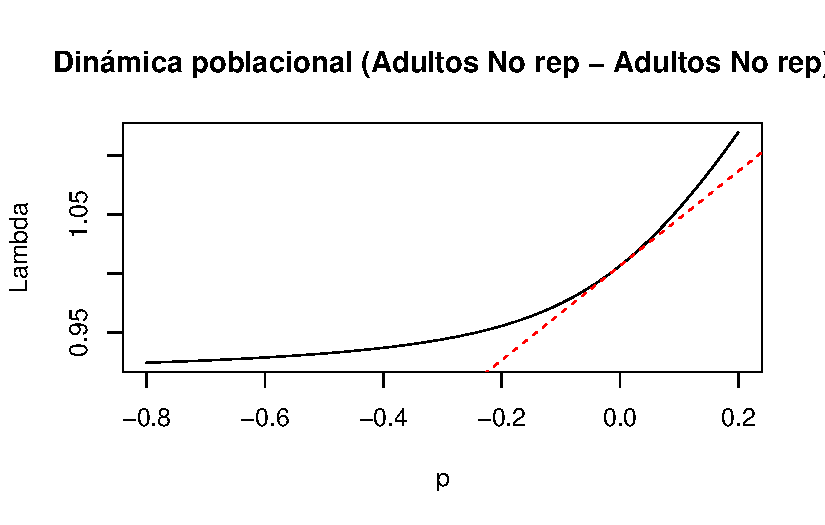
\includegraphics{113-Funciones_de_Transferencia_files/figure-pdf/unnamed-chunk-5-1.pdf}

\begin{center}\rule{0.5\linewidth}{0.5pt}\end{center}

\emph{b Elasticidad No Lineal: Efecto del Crecimiento de la Fase Juvenil
a Reproductiva {[}4,2{]} sobre λ}

En este y los siguientes ejemplos, el análisis se centra en la
estructura de perturbación y la magnitud de la perturbación, ya que son
los componentes que varían. La perturbación correspondiente al
crecimiento o tránsito de la fase juvenil a adulto reproductivo
{[}4,2{]} se define mediante los siguientes vectores y rango:

\begin{itemize}
\tightlist
\item
  \texttt{d} = c(0, 1, 0, 0)
\item
  \texttt{e} = c(0, 0, 0, 1)
\item
  \texttt{prange} = seq(0, 0.89, 0.01)
\end{itemize}

Los resultados indican que la perturbación en esta transición ejerce un
efecto no lineal sobre λ. Este efecto es positivo para el crecimiento
poblacional, especialmente en niveles altos de perturbación.

Cuando la perturbación es menor a 0.2, el comportamiento no difiere
significativamente del esperado bajo elasticidad lineal, donde las
perturbaciones son pequeñas. Por lo tanto, en este rango, el impacto
sobre λ es prácticamente nulo.

En cambio, a medida que la magnitud de la perturbación aumenta, el
efecto sobre la tasa de crecimiento se intensifica, reflejando la
naturaleza no lineal del sistema.

\begin{Shaded}
\begin{Highlighting}[]
\CommentTok{\#Entrada de la matriz a(4,2): juveniles a adultos}
\NormalTok{tf5 }\OtherTok{\textless{}{-}} \FunctionTok{tfa\_lambda}\NormalTok{(Lr1,  }\AttributeTok{d =} \FunctionTok{c}\NormalTok{(}\DecValTok{0}\NormalTok{,}\DecValTok{1}\NormalTok{,}\DecValTok{0}\NormalTok{,}\DecValTok{0}\NormalTok{), }\AttributeTok{e =} \FunctionTok{c}\NormalTok{(}\DecValTok{0}\NormalTok{,}\DecValTok{0}\NormalTok{,}\DecValTok{0}\NormalTok{,}\DecValTok{1}\NormalTok{), }\AttributeTok{prange =} \FunctionTok{seq}\NormalTok{(}\DecValTok{0}\NormalTok{,}\FloatTok{0.89}\NormalTok{,}\FloatTok{0.01}\NormalTok{))}

\CommentTok{\#Gráfica de la dinámica poblacional}
\FunctionTok{plot}\NormalTok{(tf5, }\AttributeTok{ann =} \ConstantTok{FALSE}\NormalTok{)}
\FunctionTok{title}\NormalTok{(}\AttributeTok{main =} \StringTok{"Dinámica poblacional (Juveniles {-} Adultos)"}\NormalTok{, }\AttributeTok{ylab =} \StringTok{"Lambda"}\NormalTok{, }\AttributeTok{xlab =} \StringTok{"p"}\NormalTok{)}

\CommentTok{\#Cálculo de lambda{-}max:}
\NormalTok{lambda5 }\OtherTok{\textless{}{-}} \FunctionTok{Re}\NormalTok{(}\FunctionTok{eigen}\NormalTok{(Lr1)}\SpecialCharTok{$}\NormalTok{values[}\DecValTok{1}\NormalTok{]) }

\CommentTok{\#Cálculo de la sensibilidad}
\NormalTok{sens5 }\OtherTok{\textless{}{-}} \FunctionTok{tfs\_lambda}\NormalTok{(Lr1, }\AttributeTok{d =} \FunctionTok{c}\NormalTok{(}\DecValTok{0}\NormalTok{, }\DecValTok{1}\NormalTok{, }\DecValTok{0}\NormalTok{, }\DecValTok{0}\NormalTok{), }
                         \AttributeTok{e =} \FunctionTok{c}\NormalTok{(}\DecValTok{0}\NormalTok{, }\DecValTok{0}\NormalTok{, }\DecValTok{0}\NormalTok{, }\DecValTok{1}\NormalTok{))}

\CommentTok{\#Agregar la línea, especificando el intercepto y la pendiente}
\FunctionTok{abline}\NormalTok{(lambda5, sens5, }\AttributeTok{lty =} \DecValTok{2}\NormalTok{, }\AttributeTok{col =} \StringTok{"red"}\NormalTok{)}
\end{Highlighting}
\end{Shaded}

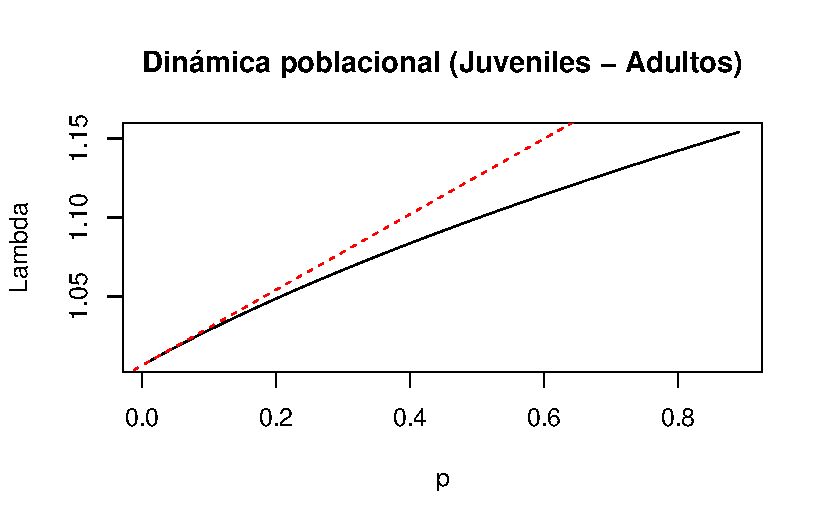
\includegraphics{113-Funciones_de_Transferencia_files/figure-pdf/unnamed-chunk-6-1.pdf}

\begin{center}\rule{0.5\linewidth}{0.5pt}\end{center}

\emph{c) Elasticidad no lineal: efecto del retroceso en estado de adulto
a no reproductivo {[}3,4{]} sobre} \(\lambda\).

En la perturbación correspondiente al retroceso o transición de la fase
adulta a adulto no reproductivo {[}3,4{]}, la ubicación vectorial se
define como:

\begin{itemize}
\tightlist
\item
  \texttt{d} = c(0, 0, 0, 1)
\item
  \texttt{e} = c(0, 0, 1, 0) y la magnitud de la perturbación se
  establece en:
\item
  \texttt{prange} = seq(0, 0.77, 0.01)
\end{itemize}

Los resultados indican que el efecto de esta perturbación sobre λ es no
lineal en niveles altos de perturbación, mientras que para
perturbaciones pequeñas (\textless{} 0.2) el comportamiento no difiere
significativamente del esperado bajo elasticidad lineal.

A medida que la magnitud de la perturbación aumenta, se observa un
efecto positivo sobre la tasa de crecimiento poblacional, lo que refleja
la importancia de esta transición en la dinámica transitoria.

\begin{Shaded}
\begin{Highlighting}[]
\CommentTok{\#Entrada de la matriz a(3,4): adultos reproductivos a NR}

\NormalTok{tf9 }\OtherTok{\textless{}{-}} \FunctionTok{tfa\_lambda}\NormalTok{(Lr1,  }\AttributeTok{d =} \FunctionTok{c}\NormalTok{(}\DecValTok{0}\NormalTok{, }\DecValTok{0}\NormalTok{, }\DecValTok{0}\NormalTok{, }\DecValTok{1}\NormalTok{),}
                       \AttributeTok{e =} \FunctionTok{c}\NormalTok{(}\DecValTok{0}\NormalTok{, }\DecValTok{0}\NormalTok{, }\DecValTok{1}\NormalTok{, }\DecValTok{0}\NormalTok{),}
                  \AttributeTok{prange =} \FunctionTok{seq}\NormalTok{(}\SpecialCharTok{{-}}\FloatTok{0.2}\NormalTok{, }\FloatTok{0.77}\NormalTok{, }\FloatTok{0.01}\NormalTok{))}

\CommentTok{\#Gráfica de la dinámica poblacional}
\FunctionTok{plot}\NormalTok{(tf9, }\AttributeTok{ann =} \ConstantTok{FALSE}\NormalTok{)}
\FunctionTok{title}\NormalTok{(}\AttributeTok{main =} \StringTok{"Dinámica poblacional (Adultos reproductivos {-} NR)"}\NormalTok{, }\AttributeTok{ylab =} \StringTok{"Lambda"}\NormalTok{, }\AttributeTok{xlab =} \StringTok{"p"}\NormalTok{)}

\CommentTok{\#Cálculo de lambda{-}max:}
\NormalTok{lambda9 }\OtherTok{\textless{}{-}} \FunctionTok{Re}\NormalTok{(}\FunctionTok{eigen}\NormalTok{(Lr1)}\SpecialCharTok{$}\NormalTok{values[}\DecValTok{1}\NormalTok{]) }

\CommentTok{\#Cálculo de la sensibilidad}
\NormalTok{sens9 }\OtherTok{\textless{}{-}} \FunctionTok{tfs\_lambda}\NormalTok{(Lr1, }\AttributeTok{d =} \FunctionTok{c}\NormalTok{(}\DecValTok{0}\NormalTok{, }\DecValTok{0}\NormalTok{, }\DecValTok{0}\NormalTok{, }\DecValTok{1}\NormalTok{), }
                        \AttributeTok{e =} \FunctionTok{c}\NormalTok{(}\DecValTok{0}\NormalTok{, }\DecValTok{0}\NormalTok{, }\DecValTok{1}\NormalTok{,  }\DecValTok{0}\NormalTok{))}

\CommentTok{\#Agregar la línea, especificando el intercepto y la pendiente}
\FunctionTok{abline}\NormalTok{(lambda9, sens9, }\AttributeTok{lty =} \DecValTok{2}\NormalTok{, }\AttributeTok{col =} \StringTok{"red"}\NormalTok{)}
\end{Highlighting}
\end{Shaded}

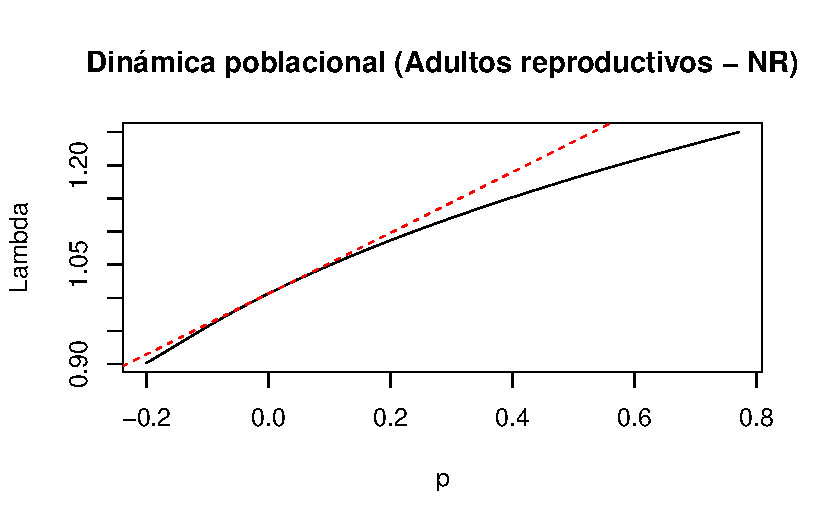
\includegraphics{113-Funciones_de_Transferencia_files/figure-pdf/unnamed-chunk-7-1.pdf}

\begin{center}\rule{0.5\linewidth}{0.5pt}\end{center}

\emph{d) Elasticidad no lineal: efecto de la contribución reproductiva
del estado de adulto a plántula {[}1,4{]} sobre} \(\lambda\).

En la perturbación correspondiente a la contribución reproductiva de
adultos hacia plántulas ({[}1,4{]}), la ubicación vectorial se define
como:

\begin{itemize}
\tightlist
\item
  \texttt{d} = c(0, 0, 0, 1)
\item
  \texttt{e} = c(1, 0, 0, 0) y la magnitud de la perturbación se
  establece en:
\item
  \texttt{prange} = seq(-0.150, 0.85, 0.01)
\end{itemize}

Los resultados indican que la perturbación en esta transición produce un
efecto lineal sobre λ. Sin embargo, la pendiente asociada a la
elasticidad no lineal es menor en comparación con la sensibilidad
lineal, lo que sugiere que el impacto de esta transición sobre la tasa
de crecimiento poblacional es más limitado de lo que se esperaría bajo
un modelo estrictamente lineal.

\begin{Shaded}
\begin{Highlighting}[]
\CommentTok{\#Entrada de la matriz a(1,4): adultos reproductivos a plántulas}

\NormalTok{tf8 }\OtherTok{\textless{}{-}} \FunctionTok{tfa\_lambda}\NormalTok{(Lr1,  }\AttributeTok{d =} \FunctionTok{c}\NormalTok{(}\DecValTok{0}\NormalTok{,}\DecValTok{0}\NormalTok{,}\DecValTok{0}\NormalTok{,}\DecValTok{1}\NormalTok{),}
                       \AttributeTok{e =} \FunctionTok{c}\NormalTok{(}\DecValTok{1}\NormalTok{,}\DecValTok{0}\NormalTok{,}\DecValTok{0}\NormalTok{,}\DecValTok{0}\NormalTok{),}
                  \AttributeTok{prange =} \FunctionTok{seq}\NormalTok{(}\SpecialCharTok{{-}}\FloatTok{0.15}\NormalTok{,}\FloatTok{0.85}\NormalTok{,}\FloatTok{0.01}\NormalTok{))}

\CommentTok{\#Gráfica de la dinámica poblacional}
\FunctionTok{plot}\NormalTok{(tf8, }\AttributeTok{ann =} \ConstantTok{FALSE}\NormalTok{)}
\FunctionTok{title}\NormalTok{(}\AttributeTok{main =} \StringTok{"Dinámica poblacional (Adultos reproductivos {-} Plántulas)"}\NormalTok{, }\AttributeTok{ylab =} \StringTok{"Lambda"}\NormalTok{, }\AttributeTok{xlab =} \StringTok{"p"}\NormalTok{)}

\CommentTok{\#Cálculo de lambda{-}max:}
\NormalTok{lambda8 }\OtherTok{\textless{}{-}} \FunctionTok{Re}\NormalTok{(}\FunctionTok{eigen}\NormalTok{(Lr1)}\SpecialCharTok{$}\NormalTok{values[}\DecValTok{1}\NormalTok{]) }

\CommentTok{\#Cálculo de la sensibilidad}
\NormalTok{sens8 }\OtherTok{\textless{}{-}} \FunctionTok{tfs\_lambda}\NormalTok{(Lr1, }\AttributeTok{d =} \FunctionTok{c}\NormalTok{(}\DecValTok{1}\NormalTok{,}\DecValTok{0}\NormalTok{,}\DecValTok{0}\NormalTok{,}\DecValTok{0}\NormalTok{), }
                         \AttributeTok{e =} \FunctionTok{c}\NormalTok{(}\DecValTok{0}\NormalTok{,}\DecValTok{0}\NormalTok{,}\DecValTok{0}\NormalTok{,}\DecValTok{1}\NormalTok{))}

\CommentTok{\#Agregar la línea, especificando el intercepto y la pendiente}
\FunctionTok{abline}\NormalTok{(lambda8, sens8, }\AttributeTok{lty =} \DecValTok{2}\NormalTok{, }\AttributeTok{col =} \StringTok{"red"}\NormalTok{)}
\end{Highlighting}
\end{Shaded}

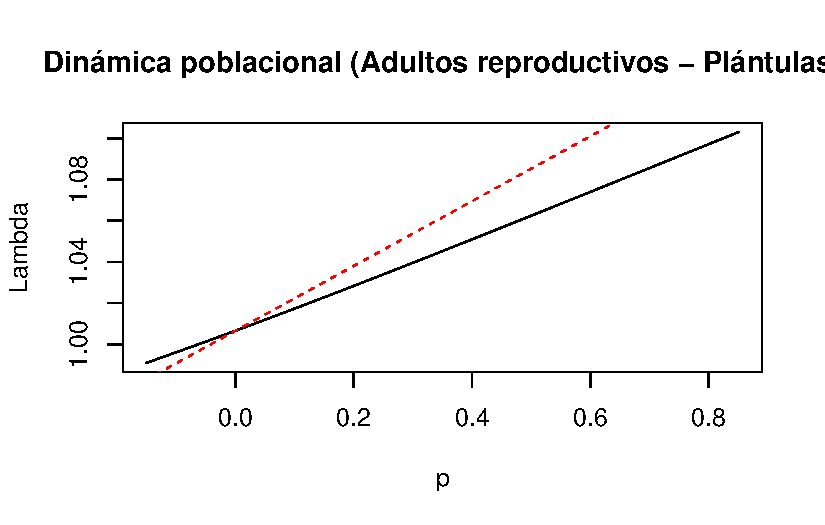
\includegraphics{113-Funciones_de_Transferencia_files/figure-pdf/unnamed-chunk-8-1.pdf}

\begin{center}\rule{0.5\linewidth}{0.5pt}\end{center}

\subsection{Elasticidad No Lineal: Uso de Toda la Matriz de Proyección
Poblacional.}\label{elasticidad-no-lineal-uso-de-toda-la-matriz-de-proyecciuxf3n-poblacional.}

La función \texttt{tfam\_lambda} permite estimar automáticamente la
elasticidad no lineal para todos los elementos distintos de cero en una
matriz poblacional, mientras que \texttt{tfmat\_lamb} genera las
gráficas correspondientes de manera automática. Stott y colaboradores
(Stott, Hodgson \& Townley, 2012b) recomiendan el uso de
\texttt{tfam\_lambda} debido a la dificultad que implica definir
manualmente la magnitud de la perturbación; por ello, este método
resulta más práctico. Sin embargo, es necesario considerar las
siguientes limitaciones:

\begin{itemize}
\tightlist
\item
  La asignación del tipo de elemento (por ejemplo, fecundidad o
  probabilidad de transición) en la matriz está predeterminada en el
  código de la función.
\item
  La magnitud de la perturbación también se calcula a partir de
  parámetros predefinidos en el código.
\end{itemize}

Estas condiciones pueden generar inconsistencias, ya que las
características de la especie analizada no siempre coinciden con los
criterios establecidos por el autor del código. Por ejemplo, en la
definición de elementos en la matriz \(A\), el código asume que todos
los valores del primer renglón corresponden a fecundidad (\(F\)). Sin
embargo, en el caso de \emph{L. rupripetala}, el elemento {[}1,1{]}
representa una probabilidad de transición (\(P\)), no una fecundidad.
Este problema se resuelve incorporando la función \texttt{elementtype},
que permite especificar el tipo de cada elemento.

Respecto a la magnitud de la perturbación, los valores predefinidos por
el autor (\texttt{Flim} = (-1, 10) y \texttt{Plim} = (-1, 10)) no pueden
modificarse. Esto implica que todos los elementos se perturban en el
mismo intervalo, lo cual es poco realista, ya que cada elemento debería
tener un rango específico según su naturaleza. En particular, el límite
superior de Plim puede generar valores mayores a 1, lo que excede la
probabilidad máxima permitida en una columna de la matriz \(A\).

Por estas razones, para controlar mejor las variables del modelo y
adaptarlo a la especie de estudio, se recomienda utilizar la función
\texttt{tfa\_lambda} y agrupar las gráficas manualmente, de forma
similar a \texttt{tfmat\_lamb}. En la última sección del capítulo se
presenta el código correspondiente en \textbf{ggplot2}.

\subsection{\texorpdfstring{Resultados del Análisis con
\texttt{tfam\_lambda}}{Resultados del Análisis con tfam\_lambda}}\label{resultados-del-anuxe1lisis-con-tfam_lambda}

En el ejemplo aplicado a \emph{L. rupripetala}, se obtuvieron los
siguientes resultados al ejecutar \texttt{tfam\_lambda} junto con la
función \texttt{elementtype}. Se generaron 10 gráficas, correspondientes
a los 10 elementos distintos de cero en la matriz \(A\). Cada gráfica se
ubica en la posición del elemento analizado. Los resultados muestran que
nueve de estas perturbaciones tienen un efecto no lineal sobre
\(\lambda\). En las gráficas, los valores del eje X (intervalo de
perturbación), \(p\) del eje Y (\(\lambda\)) no comparten la misma
escala. Las gráficas incluyen únicamente la tendencia de la elasticidad
no lineal, aunque es posible añadir la línea de sensibilidad asintótica
mediante la función \(abline\), como se hizo en los ejemplos anteriores.

En cuanto a la interpretación, se observa que la permanencia en el mismo
estado de desarrollo no sigue un patrón lineal. Además, en cuatro
elementos, aumentar la perturbación por encima de ± 0.1 genera un efecto
positivo sobre \(\lambda\). El retroceso de juvenil a no reproductivo
muestra un efecto lineal y positivo sobre \(\lambda\). Aunque el efecto
no siempre es estrictamente lineal, el impacto positivo en el
crecimiento poblacional se mantiene en las transiciones: plántula a
juvenil, juvenil a adulto reproductivo, adulto no reproductivo a
reproductivo, y en la contribución reproductiva hacia plántulas.

\begin{Shaded}
\begin{Highlighting}[]
\NormalTok{n0 }\OtherTok{\textless{}{-}} \FunctionTok{c}\NormalTok{(}\DecValTok{0}\NormalTok{, }\DecValTok{46}\NormalTok{, }\DecValTok{38}\NormalTok{, }\DecValTok{82}\NormalTok{)}
\NormalTok{etype}\OtherTok{\textless{}{-}}\FunctionTok{matrix}\NormalTok{(}\FunctionTok{c}\NormalTok{(}\StringTok{"P"}\NormalTok{, }\StringTok{"F"}\NormalTok{, }\StringTok{"F"}\NormalTok{, }\StringTok{"F"}\NormalTok{, }
                \StringTok{"P"}\NormalTok{, }\StringTok{"P"}\NormalTok{, }\StringTok{"P"}\NormalTok{, }\StringTok{"P"}\NormalTok{, }
                \StringTok{"P"}\NormalTok{, }\StringTok{"P"}\NormalTok{, }\StringTok{"P"}\NormalTok{, }\StringTok{"P"}\NormalTok{, }
                \StringTok{"P"}\NormalTok{, }\StringTok{"P"}\NormalTok{, }\StringTok{"P"}\NormalTok{, }\StringTok{"P"}\NormalTok{), }\DecValTok{4}\NormalTok{,}\DecValTok{4}\NormalTok{)}

\NormalTok{tfmat\_lamb}\OtherTok{=}\FunctionTok{tfam\_lambda}\NormalTok{(Lr1, }\AttributeTok{elementtype =}\NormalTok{ etype)}

\FunctionTok{plot}\NormalTok{(tfmat\_lamb)}
\end{Highlighting}
\end{Shaded}

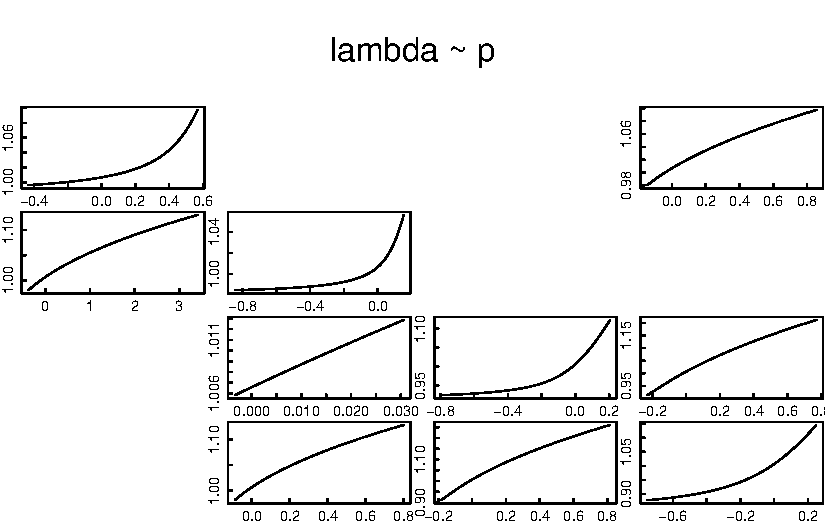
\includegraphics{113-Funciones_de_Transferencia_files/figure-pdf/transF3-1.pdf}

\begin{center}\rule{0.5\linewidth}{0.5pt}\end{center}

\section{Método de Función de Transferencia del Efecto sobre la Inercia
Poblacional}\label{muxe9todo-de-funciuxf3n-de-transferencia-del-efecto-sobre-la-inercia-poblacional}

Tras una perturbación repentina en la estructura poblacional, pueden
producirse cambios en la densidad de individuos que modifican la forma
en que la población persiste a corto plazo, fenómeno conocido como
inercia poblacional. Esto ocurre porque, después de la perturbación, las
poblaciones presentan un comportamiento inestable que genera patrones de
crecimiento distintos a los esperados en una población equivalente con
distribución estable de estado o tamaño, en adelante denominada
población estable (Stott, Hodgson \& Townley, 2012a).

Como se explicó en el capítulo sobre Elasticidad, una población estable
crece de manera exponencial a una tasa constante (\(\lambda\)) y
mantiene una estructura proporcionalmente invariable. Este patrón se
altera cuando la población no está en equilibrio estable: el crecimiento
puede fluctuar y, a corto plazo, producir densidades superiores o
inferiores a las previstas bajo una distribución estable. De igual
forma, la estructura poblacional deja de mantenerse proporcionalmente
constante (Stott, Hodgson \& Townley, 2012a). La función de
transferencia permite calcular el efecto de la elasticidad no lineal
sobre la inercia poblacional a partir de la matriz de transición de la
especie y de los cambios en el vector de estructura poblacional. Este
cálculo se expresa como el cociente entre la densidad a corto plazo de
una población no estable y la densidad correspondiente a una población
estable. Su estimación se basa en una extensión de la segunda ecuación
del método de función de transferencia aplicado a \(\lambda\) (Koons,
Holmes \& Grand, 2007; Stott, Hodgson \& Townley, 2012a), presentada
previamente en este capítulo. La extensión se formula de la siguiente
manera:

\[
\mathbf{P}_\infty = \frac{\mathbf{v}^\top \hat{\mathbf{n}}_0 \, \|\mathbf{w}\|_1}{\mathbf{v}^\top \mathbf{w}}
\] Donde

\begin{itemize}
\item
  \(\mathbf{P}_\infty\)\\
  Representa la \textbf{población proyectada en el equilibrio
  asintótico} (cuando el sistema alcanza su estructura estable).
\item
  \(\mathbf{v}^\top\)\\
  Es el \textbf{vector propio izquierdo transpuesto} asociado al
  eigenvalor dominante de la matriz de proyección. Pondera las estados
  según su contribución al crecimiento.
\item
  \(\hat{\mathbf{n}}_0\)\\
  Es el \textbf{vector inicial de población normalizado}, que indica la
  distribución inicial entre clases o estados.
\item
  \(\mathbf{w}\)\\
  Es el \textbf{vector propio derecho}, que describe la
  \textbf{distribución estable por estados} cuando la población crece a
  la tasa asintótica.
\item
  \(\|\mathbf{w}\|_1\)\\
  Es la norma L₁ del vector (\(\mathbf{w}\)), equivalente a la suma de
  sus componentes. Se usa para escalar el vector estable.
\item
  \(\mathbf{v}^\top \mathbf{w}\)\\
  Es el \textbf{producto interno entre los eigenvectores izquierdo y
  derecho}, utilizado para normalizar la expresión.
\end{itemize}

Como resultado de la ecuación, se generan valores \textgreater1 y
\textless1 que corresponden al valor de la inercia poblacional a corto
plazo. La inercia \textgreater1 indica que la población crece y se
mantiene grande, mientras que los valores \textless1 indican que decrece
y se mantiene pequeña a corto plazo (Tremblay, Raventos \& Ackerman,
2015).

El efecto de una perturbación en la inercia poblacional a través del
método de función de transferencia se evalúa aplicando las funciones
\textbf{tfa\_inertia} o \textbf{tfam\_inertia} del paquete
\textbf{popdemo} de \textbf{R} (Stott, Hodgson \& Townley, 2012a). La
primera calcula la inercia poblacional al modificar un elemento de la
estructura poblacional, mientras que la segunda estima este parámetro al
modificar todos los elementos de la estructura poblacional de forma
automática.

\section{Cambios en la estructura poblacional y su efecto en la inercia
poblacional.}\label{cambios-en-la-estructura-poblacional-y-su-efecto-en-la-inercia-poblacional.}

Tremblay y colaboradores (Tremblay, Raventos \& Ackerman, 2015) usaron
las funciones \textbf{tfa\_inertia} y \textbf{tfam\_inertia} para
modelar la relación no lineal entre una perturbación, o manipulación en
la estructura poblacional, y la inercia del crecimiento poblacional de
\emph{L. rupripetala}. Dado que la persistencia de una población puede
evaluarse bajo distintos escenarios si se modifica un elemento de la
matriz de transición, estos autores evaluaron la inercia poblacional
considerando los siguientes supuestos:

\begin{enumerate}
\def\labelenumi{\alph{enumi})}
\item
  Un caso específico del ciclo de vida, por ejemplo el elemento con la
  elasticidad más alta.
\item
  Cambios en todas y cada una de los elementos de la matriz \(A\).
\item
  Cambios en la última y la primera categoría de estado en la población.
\item
  Tomando en cuenta la estructura estable inicial, que evalúa la
  persistencia de la población si se encontrara en el equilibrio
  (Tremblay, Raventos \& Ackerman, 2015).
\end{enumerate}

Con base en estos escenarios, a continuación se describe cómo aplicar
\textbf{tfa\_inertia} y \textbf{tfam\_inertia}.

\subsection{\texorpdfstring{\emph{Elasticidad no lineal a través de}
\textbf{tfa\_inertia}.}{Elasticidad no lineal a través de tfa\_inertia.}}\label{elasticidad-no-lineal-a-travuxe9s-de-tfa_inertia.}

El primer escenario: un caso específico del ciclo de vida, permitirá
ejemplificar el uso de la función \textbf{tfa\_inertia}. En este se
evalúa el efecto de la estasis o permanencia en el estado no
reproductivo {[}3,3{]} sobre la inercia poblacional y fue seleccionado
porque presenta el valor más alto de elasticidad. En el cálculo se usan
los siguientes argumentos para esta función: la matriz de transición de
la población \emph{Lr1}; indicamos el vector de la estructura
poblacional, la estructura de perturbación (elemento de la matriz a
perturbar) y la magnitud de la perturbación la estructura de
perturbación o \texttt{prange} = seq(-0.7954, 0.0205, 0.01). En el
recuadro se presenta el código correspondiente para su estimación.

Como resultado se genera una gráfica en la que se aprecia el
comportamiento de la inercia o persistencia poblacional a corto plazo
ante una perturbación. Esta respuesta se da de forma proporcional y de
manera creciente, teniendo como puntos extremos en el eje \emph{x} la
perturbación mínima y la máxima. La línea roja representa la elasticidad
a perturbación cero y la línea negra la función de transferencia de la
inercia poblacional ante cambios en la permanencia en la fase de adulto
no reproductivo.

La tendencia de la elasticidad no lineal sugiere que cualquier aumento
en la estasis en la categoría de adulto no reproductivo provocará una
disminución en el valor de la inercia poblacional a corto plazo.
Tremblay y colaboradores (Tremblay, Raventos \& Ackerman, 2015)
presentan en la figura 4 los resultados de los casos en que las
elasticidades fueron mayores.

\begin{Shaded}
\begin{Highlighting}[]
\NormalTok{n0 }\OtherTok{\textless{}{-}} \FunctionTok{c}\NormalTok{(}\DecValTok{0}\NormalTok{, }\DecValTok{46}\NormalTok{, }\DecValTok{38}\NormalTok{, }\DecValTok{82}\NormalTok{)}

\NormalTok{tf2}\OtherTok{\textless{}{-}}\FunctionTok{tfa\_inertia}\NormalTok{(Lr1, }\AttributeTok{vector=}\NormalTok{n0, }\AttributeTok{d=}\FunctionTok{c}\NormalTok{(}\DecValTok{0}\NormalTok{,}\DecValTok{0}\NormalTok{,}\DecValTok{1}\NormalTok{,}\DecValTok{0}\NormalTok{), }\AttributeTok{e=}\FunctionTok{c}\NormalTok{(}\DecValTok{0}\NormalTok{,}\DecValTok{0}\NormalTok{,}\DecValTok{1}\NormalTok{,}\DecValTok{0}\NormalTok{), }\AttributeTok{prange=}\FunctionTok{seq}\NormalTok{(}\SpecialCharTok{{-}}\FloatTok{0.8}\NormalTok{,}\FloatTok{0.2}\NormalTok{,}\FloatTok{0.01}\NormalTok{)) }\CommentTok{\# el efecto de perturbación de la transición de no reproductivo a adulto reproductivo}


\FunctionTok{plot}\NormalTok{(tf2, }\AttributeTok{main=}\StringTok{"Inercia poblacional"}\NormalTok{,}\AttributeTok{cex.axis=}\FloatTok{1.4}\NormalTok{,}\AttributeTok{cex.lab=}\FloatTok{1.5}\NormalTok{) }\CommentTok{\# gráfica de la inercia poblacional}

\NormalTok{inertia}\OtherTok{\textless{}{-}}\FunctionTok{inertia}\NormalTok{(Lr1, }\AttributeTok{vector=}\NormalTok{n0)}

\NormalTok{sens2}\OtherTok{\textless{}{-}}\FunctionTok{tfs\_inertia}\NormalTok{(Lr1, }\AttributeTok{vector=}\NormalTok{n0, }\AttributeTok{d=}\FunctionTok{c}\NormalTok{(}\DecValTok{0}\NormalTok{,}\DecValTok{0}\NormalTok{,}\DecValTok{1}\NormalTok{,}\DecValTok{0}\NormalTok{), }\AttributeTok{e=}\FunctionTok{c}\NormalTok{(}\DecValTok{0}\NormalTok{,}\DecValTok{0}\NormalTok{,}\DecValTok{1}\NormalTok{,}\DecValTok{0}\NormalTok{), }\AttributeTok{tolerance=}\FloatTok{1e{-}5}\NormalTok{) }\CommentTok{\# el efecto de sensibilidad de la inercia poblacional}
\FunctionTok{abline}\NormalTok{(inertia, sens2, }\AttributeTok{lty=}\DecValTok{2}\NormalTok{, }\AttributeTok{col=}\StringTok{"red"}\NormalTok{) }\CommentTok{\# Para añadir el efecto lineal }
\end{Highlighting}
\end{Shaded}

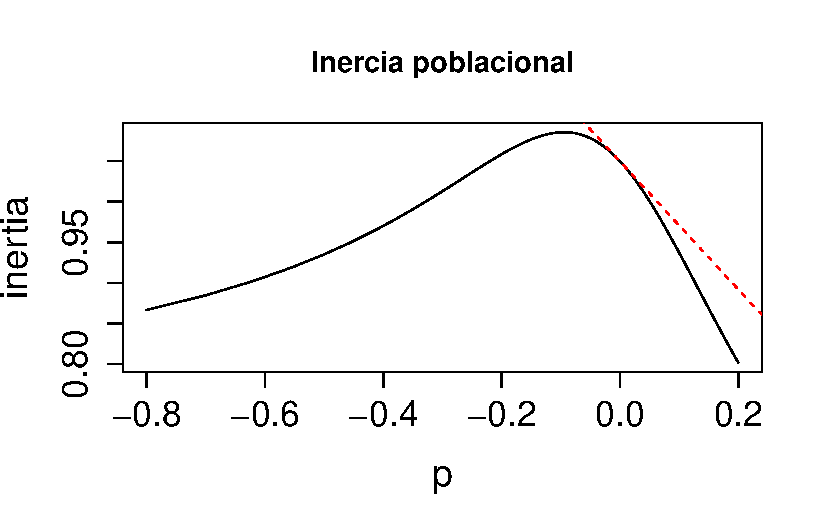
\includegraphics{113-Funciones_de_Transferencia_files/figure-pdf/unnamed-chunk-9-1.pdf}

\begin{center}\rule{0.5\linewidth}{0.5pt}\end{center}

\subsection{\texorpdfstring{\emph{Elasticidad no lineal a través de}
\textbf{tfam\_inertia}.}{Elasticidad no lineal a través de tfam\_inertia.}}\label{elasticidad-no-lineal-a-travuxe9s-de-tfam_inertia.}

En el cálculo de inercia poblacional se puede optar por evaluar los
efectos de todas las entradas de la matriz con valor \textgreater0. La
función \textbf{matA} ofrece esta opción y su uso se ejemplificará a
través de los tres escenarios faltantes (b, c y d).

En este cálculo de la inercia poblacional se usan los siguientes
argumentos para esta función: la matriz de transición de la población
\emph{Lr1}; el vector de la estructura poblacional, y, al igual que en
\textbf{tfam\_lambda}, se hacen los ajustes de los tipos de elementos en
la matriz con \textbf{elementtype} y se mantienen los límite mínimo y
máximo de las funciones \texttt{Plim} y \texttt{Flim} definidos por el
autor del código.

A continuación se proyecta la persistencia de \emph{L. rupripetala} para
los tres escenarios faltantes: Perturbación de todo el ciclo de vida,
concentración de individuos en la última y primera categoría, y, la
estructura estable inicial.

\begin{itemize}
\tightlist
\item
  \emph{Perturbación de todo el ciclo de vida}. Los resultados de la
  simulación de perturbación de todas y cada uno de los elementos de la
  matriz: reproducción, crecimiento y supervivencia, sugieren que la
  permanencia en las cuatro fases del ciclo de vida de \emph{L.
  rupripetala} tienen un impacto negativo en la inercia poblacional.
  Cualquier aumento en la estasis en la permanencia en alguno de los
  cuatro estados provocará una disminución en la densidad de la
  población a corto plazo.
\end{itemize}

A excepción del tránsito de adulto no reproductivo a reproductivo, el
tránsito a un estado superior tiene un efecto positivo en la inercia
poblacional. Lo mismo sucede con la retrogresión de adultos
reproductivos a no reproductivos y en la contribución reproductiva de
adultos a plántulas.

\begin{Shaded}
\begin{Highlighting}[]
\CommentTok{\#Definir márgenes}
\FunctionTok{par}\NormalTok{(}\AttributeTok{mfrow =} \FunctionTok{c}\NormalTok{(}\DecValTok{4}\NormalTok{,}\DecValTok{4}\NormalTok{))}
\FunctionTok{par}\NormalTok{(}\AttributeTok{mfg =} \FunctionTok{c}\NormalTok{(}\DecValTok{1}\NormalTok{,}\DecValTok{1}\NormalTok{))}

\CommentTok{\#Gráficas de la función de transferencia de la inercia en el ciclo de vida de L. rubripetala (población 1)}

\NormalTok{etype}\OtherTok{\textless{}{-}}\FunctionTok{matrix}\NormalTok{(}\FunctionTok{c}\NormalTok{(}\StringTok{"P"}\NormalTok{, }\StringTok{"F"}\NormalTok{, }\StringTok{"F"}\NormalTok{, }\StringTok{"F"}\NormalTok{, }
                \StringTok{"P"}\NormalTok{, }\StringTok{"P"}\NormalTok{, }\StringTok{"P"}\NormalTok{, }\StringTok{"P"}\NormalTok{, }
                \StringTok{"P"}\NormalTok{, }\StringTok{"P"}\NormalTok{, }\StringTok{"P"}\NormalTok{, }\StringTok{"P"}\NormalTok{, }
                \StringTok{"P"}\NormalTok{, }\StringTok{"P"}\NormalTok{, }\StringTok{"P"}\NormalTok{, }\StringTok{"P"}\NormalTok{), }\DecValTok{4}\NormalTok{,}\DecValTok{4}\NormalTok{)}

\NormalTok{tfmatriz }\OtherTok{\textless{}{-}} \FunctionTok{tfam\_inertia}\NormalTok{(Lr1, }\AttributeTok{elementtype =}\NormalTok{ etype, }\AttributeTok{vector =}\NormalTok{ nLr0)}

\FunctionTok{plot}\NormalTok{(tfmatriz,  }\AttributeTok{xlab=}\StringTok{"p"}\NormalTok{, }\AttributeTok{ylab=}\StringTok{"Inercia"}\NormalTok{, }\AttributeTok{cex.axis=}\FloatTok{1.4}\NormalTok{, }\AttributeTok{cex.lab=}\FloatTok{1.5}\NormalTok{)}
\end{Highlighting}
\end{Shaded}

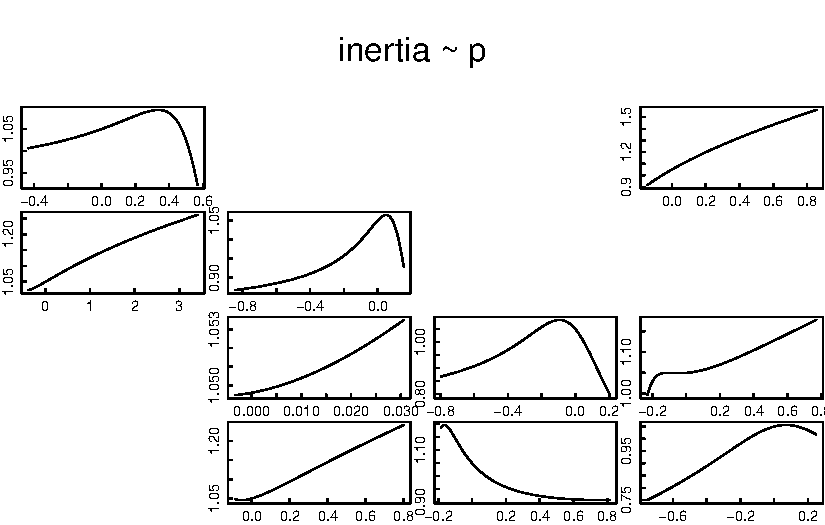
\includegraphics{113-Funciones_de_Transferencia_files/figure-pdf/unnamed-chunk-10-1.pdf}

\begin{center}\rule{0.5\linewidth}{0.5pt}\end{center}

\begin{itemize}
\item
  \emph{Última y primera categoría}. La función de transferencia de la
  inercia fue estimada al suponer que la población se encuentra
  concentrada en:

  \emph{i) la categoría de adulto reproductivo (Upper bound)}.
\end{itemize}

El código para el cálculo de la inercia poblacional se presenta en el
siguiente recuadro. En este se supone que la población está representada
por el último estado del ciclo de vida. Los resultados de la gráfica
(extremo inferior derecho) sugieren que cuando todos los individuos de
\emph{L. rubripetala} se encuentran en la fase de adulto reproductivo,
la inercia poblacional a corto plazo será mayor a 1.4, lo que sugiere
que la población puede crecer por más del 40\% antes de alcanzar la tasa
constante de crecimiento poblacional. Asimismo, estos resultados indican
que los adultos reproductivos tienen un alto impacto positivo sobre la
tasa de crecimiento poblacional, a excepción de la transición juveniles
a adultos no reproductivos.

\begin{Shaded}
\begin{Highlighting}[]
\NormalTok{etype}\OtherTok{\textless{}{-}}\FunctionTok{matrix}\NormalTok{(}\FunctionTok{c}\NormalTok{(}\StringTok{"P"}\NormalTok{, }\StringTok{"F"}\NormalTok{, }\StringTok{"F"}\NormalTok{, }\StringTok{"F"}\NormalTok{,}
                \StringTok{"P"}\NormalTok{, }\StringTok{"P"}\NormalTok{, }\StringTok{"P"}\NormalTok{, }\StringTok{"P"}\NormalTok{,}
                \StringTok{"P"}\NormalTok{, }\StringTok{"P"}\NormalTok{, }\StringTok{"P"}\NormalTok{, }\StringTok{"P"}\NormalTok{, }
                \StringTok{"P"}\NormalTok{, }\StringTok{"P"}\NormalTok{, }\StringTok{"P"}\NormalTok{, }\StringTok{"P"}\NormalTok{), }\DecValTok{4}\NormalTok{,}\DecValTok{4}\NormalTok{)}

\NormalTok{tfmatU}\OtherTok{=}\FunctionTok{tfam\_inertia}\NormalTok{(Lr1, }\AttributeTok{elementtype =}\NormalTok{ etype, }\AttributeTok{bound =} \StringTok{"upper"}\NormalTok{) }\CommentTok{\# donde todos los individuos están en el ultimo estadio}

\FunctionTok{plot}\NormalTok{(tfmatU, }\AttributeTok{cex.axis=}\FloatTok{1.4}\NormalTok{, }\AttributeTok{cex.lab=}\FloatTok{1.5}\NormalTok{) }\CommentTok{\# gráfica de la inercia poblacional}
\end{Highlighting}
\end{Shaded}

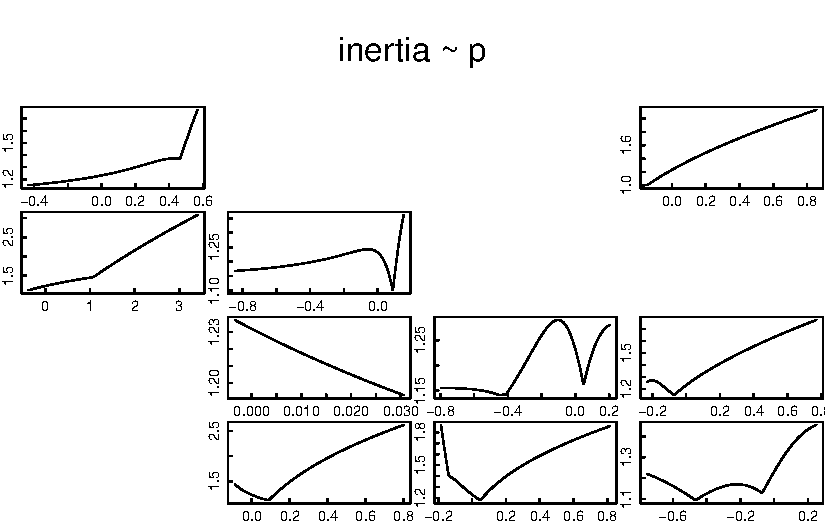
\includegraphics{113-Funciones_de_Transferencia_files/figure-pdf/unnamed-chunk-11-1.pdf}

\begin{center}\rule{0.5\linewidth}{0.5pt}\end{center}

\emph{ii) la categoría de plántulas (Lower bound)}.

El código del cálculo de la inercia poblacional al suponer que la
población está dominada por el primer estado del ciclo de vida se
presenta en el siguiente recuadro. Los resultados de la primera gráfica
(extremo superior derecho) sugieren que al suponer que todos los
individuos de \emph{L. rubripetala} se concentran en el límite inferior,
la inercia poblacional a corto plazo es de 0.7, lo que sugiere que la
población puede reducir hasta un 30\% antes de alcanzar la tasa
constante de crecimiento poblacional. En este escenario se reconoce que
la dominancia de las plántulas en la población tiene un impacto negativo
en el crecimiento de la población a corto plazo, ya que es todos los
casos la \(lambda\) poblacional está por debajo de 1.

\begin{Shaded}
\begin{Highlighting}[]
\NormalTok{tfmatL}\OtherTok{=}\FunctionTok{tfam\_inertia}\NormalTok{(Lr1, }\AttributeTok{elementtype =}\NormalTok{ etype, }\AttributeTok{bound =} \StringTok{"lower"}\NormalTok{) }\CommentTok{\# donde todos los individuos están en el primer estadio}

\FunctionTok{plot}\NormalTok{(tfmatL)}
\end{Highlighting}
\end{Shaded}

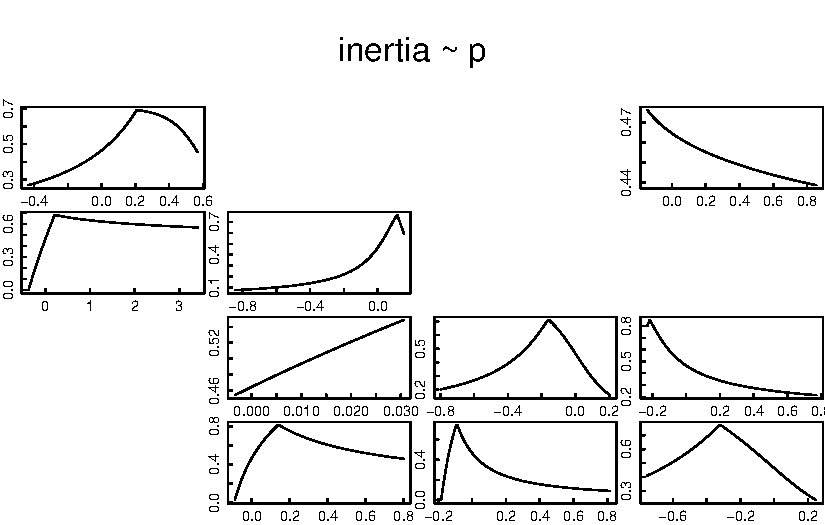
\includegraphics{113-Funciones_de_Transferencia_files/figure-pdf/unnamed-chunk-12-1.pdf}

\begin{center}\rule{0.5\linewidth}{0.5pt}\end{center}

\emph{c) la estructura estable inicial}.

En el siguiente recuadro se presenta el código del cálculo de la inercia
poblacional para una población que se encuentra en su estructura estable
y, por tanto, en equilibrio. Los resultados de la primera gráfica
(extremo superior derecho) sugieren que la fecundidad tiene el mayor
impacto positivo en la dinámica transitoria si la población se encuentra
en en equilibrio. En estas condiciones, duplicar la fecundidad aumenta
significativamente el tamaño de la población a corto plazo.

\begin{Shaded}
\begin{Highlighting}[]
\NormalTok{n0 }\OtherTok{\textless{}{-}} \FunctionTok{c}\NormalTok{(}\DecValTok{0}\NormalTok{, }\DecValTok{46}\NormalTok{, }\DecValTok{38}\NormalTok{, }\DecValTok{82}\NormalTok{)}

\NormalTok{stable }\OtherTok{\textless{}{-}}\NormalTok{ popbio}\SpecialCharTok{::}\FunctionTok{stable.stage}\NormalTok{(Lr1) }\CommentTok{\# calcular el estado estable de la matriz Lr1}


\NormalTok{tfmat\_I}\OtherTok{=}\FunctionTok{tfam\_inertia}\NormalTok{(Lr1, }\AttributeTok{elementtype =}\NormalTok{ etype, }\AttributeTok{vector =}\NormalTok{ stable) }\CommentTok{\# donde los individuos están en la estructura de población inicial}

\FunctionTok{plot}\NormalTok{(tfmat\_I)}
\end{Highlighting}
\end{Shaded}

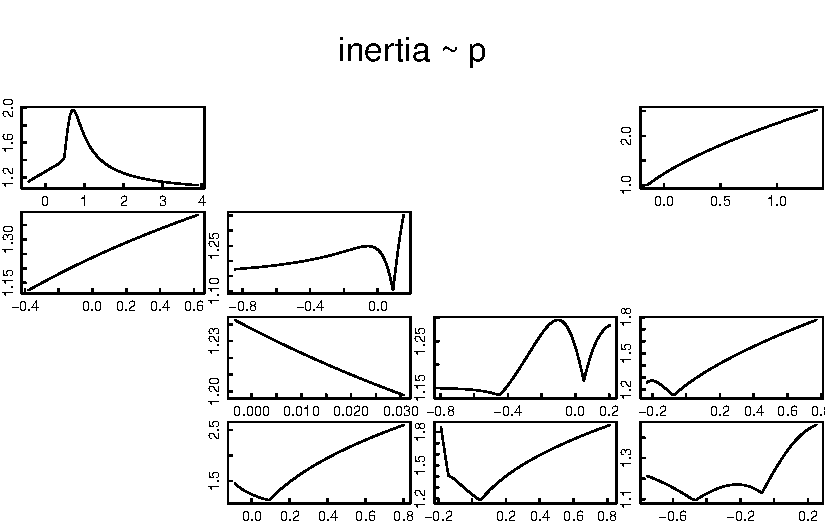
\includegraphics{113-Funciones_de_Transferencia_files/figure-pdf/transF5-1.pdf}

\begin{center}\rule{0.5\linewidth}{0.5pt}\end{center}

\section{Contenido extra}\label{contenido-extra}

\subsection{Uso de ggplot2 para la matriz de figuras generadas con la
función de
transferencia}\label{uso-de-ggplot2-para-la-matriz-de-figuras-generadas-con-la-funciuxf3n-de-transferencia}

En esta sección se presenta el código con \emph{ggplot2} para agrupar en
una sola gráfica las 10 figuras generadas una por una para la matriz
\(A\) (ver \emph{Estimación de la elasticidad lineal por elemento
perturbado}) y las cuales ilustran el efecto de la perturbación de cada
elemento distinto de 0 sobre la inercia poblacional. Esta sección
resulta de gran utilidad y es una alternativa muy buena al uso de
\textbf{tfam\_lambda} y \textbf{tfam\_inertia}, ya que se evitarán los
valores predeterminados en el código original para \texttt{Flim} y
\texttt{Plim}, permitiendo la descripción del comportamiento de la
especie con mayor certeza y basada en sus parámetros poblacionales
propios.

Finalmente, cabe señalar que con los ajustes necesarios, este código
puede ser aplicado a los resultados elemento por elemento de
\textbf{tfa\_inertia}.

\begin{Shaded}
\begin{Highlighting}[]
\NormalTok{tf1df}\OtherTok{=}\FunctionTok{as.data.frame}\NormalTok{(tf1)}
\NormalTok{tf1tf}\OtherTok{=}\NormalTok{ggplot2}\SpecialCharTok{::}\FunctionTok{ggplot}\NormalTok{() }\SpecialCharTok{+}
\NormalTok{  ggplot2}\SpecialCharTok{::}\FunctionTok{geom\_line}\NormalTok{(}\AttributeTok{data =}\NormalTok{ tf1df, }\FunctionTok{aes}\NormalTok{(}\AttributeTok{x =}\NormalTok{ p, }\AttributeTok{y =}\NormalTok{ lambda), }\AttributeTok{color =} \StringTok{"blue"}\NormalTok{) }\SpecialCharTok{+}
\NormalTok{  ggplot2}\SpecialCharTok{::}\FunctionTok{geom\_abline}\NormalTok{(}\AttributeTok{slope =}\NormalTok{ sens1, }\AttributeTok{intercept =}\NormalTok{ lambda1, }\AttributeTok{linetype =} \StringTok{"dashed"}\NormalTok{, }\AttributeTok{color =} \StringTok{"red"}\NormalTok{) }\SpecialCharTok{+}
  \CommentTok{\#ggplot2::labs(title = "P {-} P", x = "p", y = "Lambda") +}
\NormalTok{  ggplot2}\SpecialCharTok{::}\FunctionTok{theme\_minimal}\NormalTok{()}\SpecialCharTok{+}
  \FunctionTok{ylab}\NormalTok{(}\StringTok{""}\NormalTok{)}\SpecialCharTok{+}\FunctionTok{xlab}\NormalTok{(}\StringTok{""}\NormalTok{)}\SpecialCharTok{+}
  \FunctionTok{theme}\NormalTok{(}\AttributeTok{axis.text.x =} \FunctionTok{element\_text}\NormalTok{(}\AttributeTok{angle =} \DecValTok{45}\NormalTok{, }\AttributeTok{size=}\DecValTok{6}\NormalTok{),}
        \AttributeTok{axis.text.y =} \FunctionTok{element\_text}\NormalTok{(}\AttributeTok{size=}\DecValTok{6}\NormalTok{))}
  


\NormalTok{tf2df}\OtherTok{=}\FunctionTok{as.data.frame}\NormalTok{(tf2)}
\NormalTok{tf2tf}\OtherTok{=}\NormalTok{ggplot2}\SpecialCharTok{::}\FunctionTok{ggplot}\NormalTok{() }\SpecialCharTok{+}
\NormalTok{  ggplot2}\SpecialCharTok{::}\FunctionTok{geom\_line}\NormalTok{(}\AttributeTok{data =}\NormalTok{ tf2df, }\FunctionTok{aes}\NormalTok{(}\AttributeTok{x =}\NormalTok{ p, }\AttributeTok{y =}\NormalTok{ lambda), }\AttributeTok{color =} \StringTok{"blue"}\NormalTok{) }\SpecialCharTok{+}
\NormalTok{  ggplot2}\SpecialCharTok{::}\FunctionTok{geom\_abline}\NormalTok{(}\AttributeTok{slope =}\NormalTok{ sens2, }\AttributeTok{intercept =}\NormalTok{ lambda2, }\AttributeTok{linetype =} \StringTok{"dashed"}\NormalTok{, }\AttributeTok{color =} \StringTok{"red"}\NormalTok{) }\SpecialCharTok{+}
 \CommentTok{\# ggplot2::labs(title = "P {-} J", x = "p", y = "Lambda") +}
\NormalTok{  ggplot2}\SpecialCharTok{::}\FunctionTok{theme\_minimal}\NormalTok{()}\SpecialCharTok{+}
  \FunctionTok{ylab}\NormalTok{(}\StringTok{""}\NormalTok{)}\SpecialCharTok{+}\FunctionTok{xlab}\NormalTok{(}\StringTok{""}\NormalTok{)}\SpecialCharTok{+}
  \FunctionTok{theme}\NormalTok{(}\AttributeTok{axis.text.x =} \FunctionTok{element\_text}\NormalTok{(}\AttributeTok{angle =} \DecValTok{45}\NormalTok{, }\AttributeTok{size=}\DecValTok{6}\NormalTok{),}
        \AttributeTok{axis.text.y =} \FunctionTok{element\_text}\NormalTok{(}\AttributeTok{size=}\DecValTok{6}\NormalTok{))}

\NormalTok{tf3df}\OtherTok{=}\FunctionTok{as.data.frame}\NormalTok{(tf3)}
\NormalTok{tf3tf}\OtherTok{=}\NormalTok{ggplot2}\SpecialCharTok{::}\FunctionTok{ggplot}\NormalTok{() }\SpecialCharTok{+}
\NormalTok{  ggplot2}\SpecialCharTok{::}\FunctionTok{geom\_line}\NormalTok{(}\AttributeTok{data =}\NormalTok{ tf3df, }\FunctionTok{aes}\NormalTok{(}\AttributeTok{x =}\NormalTok{ p, }\AttributeTok{y =}\NormalTok{ lambda), }\AttributeTok{color =} \StringTok{"blue"}\NormalTok{) }\SpecialCharTok{+}
\NormalTok{  ggplot2}\SpecialCharTok{::}\FunctionTok{geom\_abline}\NormalTok{(}\AttributeTok{slope =}\NormalTok{ sens3, }\AttributeTok{intercept =}\NormalTok{ lambda3, }\AttributeTok{linetype =} \StringTok{"dashed"}\NormalTok{, }\AttributeTok{color =} \StringTok{"red"}\NormalTok{) }\SpecialCharTok{+}
  \CommentTok{\#ggplot2::labs(title = "J {-} J", x = "p", y = "Lambda") +}
\NormalTok{  ggplot2}\SpecialCharTok{::}\FunctionTok{theme\_minimal}\NormalTok{()}\SpecialCharTok{+}
  \FunctionTok{ylab}\NormalTok{(}\StringTok{""}\NormalTok{)}\SpecialCharTok{+}\FunctionTok{xlab}\NormalTok{(}\StringTok{""}\NormalTok{)}\SpecialCharTok{+}
  \FunctionTok{theme}\NormalTok{(}\AttributeTok{axis.text.x =} \FunctionTok{element\_text}\NormalTok{(}\AttributeTok{angle =} \DecValTok{45}\NormalTok{, }\AttributeTok{size=}\DecValTok{6}\NormalTok{),}
        \AttributeTok{axis.text.y =} \FunctionTok{element\_text}\NormalTok{(}\AttributeTok{size=}\DecValTok{6}\NormalTok{))}

\NormalTok{tf4df}\OtherTok{=}\FunctionTok{as.data.frame}\NormalTok{(tf4)}

\NormalTok{tf4tf}\OtherTok{=}\NormalTok{ggplot2}\SpecialCharTok{::}\FunctionTok{ggplot}\NormalTok{() }\SpecialCharTok{+}
\NormalTok{  ggplot2}\SpecialCharTok{::}\FunctionTok{geom\_line}\NormalTok{(}\AttributeTok{data =}\NormalTok{ tf4df, }\FunctionTok{aes}\NormalTok{(}\AttributeTok{x =}\NormalTok{ p, }\AttributeTok{y =}\NormalTok{ lambda), }\AttributeTok{color =} \StringTok{"blue"}\NormalTok{) }\SpecialCharTok{+}
\NormalTok{  ggplot2}\SpecialCharTok{::}\FunctionTok{geom\_abline}\NormalTok{(}\AttributeTok{slope =}\NormalTok{ sens4, }\AttributeTok{intercept =}\NormalTok{ lambda4, }\AttributeTok{linetype =} \StringTok{"dashed"}\NormalTok{, }\AttributeTok{color =} \StringTok{"red"}\NormalTok{) }\SpecialCharTok{+}
 \CommentTok{\# ggplot2::labs(title = "J {-} NR", x = "p", y = "Lambda") +}
\NormalTok{  ggplot2}\SpecialCharTok{::}\FunctionTok{theme\_minimal}\NormalTok{()}\SpecialCharTok{+}
  \FunctionTok{ylab}\NormalTok{(}\StringTok{""}\NormalTok{)}\SpecialCharTok{+}\FunctionTok{xlab}\NormalTok{(}\StringTok{""}\NormalTok{)}\SpecialCharTok{+}
  \FunctionTok{theme}\NormalTok{(}\AttributeTok{axis.text.x =} \FunctionTok{element\_text}\NormalTok{(}\AttributeTok{angle =} \DecValTok{45}\NormalTok{, }\AttributeTok{size=}\DecValTok{6}\NormalTok{),}
        \AttributeTok{axis.text.y =} \FunctionTok{element\_text}\NormalTok{(}\AttributeTok{size=}\DecValTok{6}\NormalTok{))}

\NormalTok{tf5df}\OtherTok{=}\FunctionTok{as.data.frame}\NormalTok{(tf5)}

\NormalTok{tf5tf}\OtherTok{=}\NormalTok{ggplot2}\SpecialCharTok{::}\FunctionTok{ggplot}\NormalTok{() }\SpecialCharTok{+}
\NormalTok{  ggplot2}\SpecialCharTok{::}\FunctionTok{geom\_line}\NormalTok{(}\AttributeTok{data =}\NormalTok{ tf5df, }\FunctionTok{aes}\NormalTok{(}\AttributeTok{x =}\NormalTok{ p, }\AttributeTok{y =}\NormalTok{ lambda), }\AttributeTok{color =} \StringTok{"blue"}\NormalTok{) }\SpecialCharTok{+}
\NormalTok{  ggplot2}\SpecialCharTok{::}\FunctionTok{geom\_abline}\NormalTok{(}\AttributeTok{slope =}\NormalTok{ sens5, }\AttributeTok{intercept =}\NormalTok{ lambda5, }\AttributeTok{linetype =} \StringTok{"dashed"}\NormalTok{, }\AttributeTok{color =} \StringTok{"red"}\NormalTok{) }\SpecialCharTok{+}
 \CommentTok{\# ggplot2::labs(title = "J {-} A", x = "p", y = "Lambda") +}
\NormalTok{  ggplot2}\SpecialCharTok{::}\FunctionTok{theme\_minimal}\NormalTok{()}\SpecialCharTok{+}
  \FunctionTok{ylab}\NormalTok{(}\StringTok{""}\NormalTok{)}\SpecialCharTok{+}\FunctionTok{xlab}\NormalTok{(}\StringTok{""}\NormalTok{)}\SpecialCharTok{+}
  \FunctionTok{theme}\NormalTok{(}\AttributeTok{axis.text.x =} \FunctionTok{element\_text}\NormalTok{(}\AttributeTok{angle =} \DecValTok{45}\NormalTok{, }\AttributeTok{size=}\DecValTok{6}\NormalTok{),}
        \AttributeTok{axis.text.y =} \FunctionTok{element\_text}\NormalTok{(}\AttributeTok{size=}\DecValTok{6}\NormalTok{))}

\NormalTok{tf6df}\OtherTok{=}\FunctionTok{as.data.frame}\NormalTok{(tf6)}

\NormalTok{tf6tf}\OtherTok{=}\NormalTok{ggplot2}\SpecialCharTok{::}\FunctionTok{ggplot}\NormalTok{() }\SpecialCharTok{+}
\NormalTok{  ggplot2}\SpecialCharTok{::}\FunctionTok{geom\_line}\NormalTok{(}\AttributeTok{data =}\NormalTok{ tf6df, }\FunctionTok{aes}\NormalTok{(}\AttributeTok{x =}\NormalTok{ p, }\AttributeTok{y =}\NormalTok{ lambda), }\AttributeTok{color =} \StringTok{"blue"}\NormalTok{) }\SpecialCharTok{+}
\NormalTok{  ggplot2}\SpecialCharTok{::}\FunctionTok{geom\_abline}\NormalTok{(}\AttributeTok{slope =}\NormalTok{ sens6, }\AttributeTok{intercept =}\NormalTok{ lambda6, }\AttributeTok{linetype =} \StringTok{"dashed"}\NormalTok{, }\AttributeTok{color =} \StringTok{"red"}\NormalTok{) }\SpecialCharTok{+}
  \CommentTok{\#ggplot2::labs(title = "NR {-} NR", x = "p", y = "Lambda") +}
\NormalTok{  ggplot2}\SpecialCharTok{::}\FunctionTok{theme\_minimal}\NormalTok{()}\SpecialCharTok{+}
  \FunctionTok{ylab}\NormalTok{(}\StringTok{""}\NormalTok{)}\SpecialCharTok{+}\FunctionTok{xlab}\NormalTok{(}\StringTok{""}\NormalTok{)}\SpecialCharTok{+}
  \FunctionTok{theme}\NormalTok{(}\AttributeTok{axis.text.x =} \FunctionTok{element\_text}\NormalTok{(}\AttributeTok{angle =} \DecValTok{45}\NormalTok{, }\AttributeTok{size=}\DecValTok{6}\NormalTok{),}
        \AttributeTok{axis.text.y =} \FunctionTok{element\_text}\NormalTok{(}\AttributeTok{size=}\DecValTok{6}\NormalTok{))}

\NormalTok{tf7df}\OtherTok{=}\FunctionTok{as.data.frame}\NormalTok{(tf7)}

\NormalTok{tf7tf}\OtherTok{=}\NormalTok{ggplot2}\SpecialCharTok{::}\FunctionTok{ggplot}\NormalTok{() }\SpecialCharTok{+}
\NormalTok{  ggplot2}\SpecialCharTok{::}\FunctionTok{geom\_line}\NormalTok{(}\AttributeTok{data =}\NormalTok{ tf7df, }\FunctionTok{aes}\NormalTok{(}\AttributeTok{x =}\NormalTok{ p, }\AttributeTok{y =}\NormalTok{ lambda), }\AttributeTok{color =} \StringTok{"blue"}\NormalTok{) }\SpecialCharTok{+}
\NormalTok{  ggplot2}\SpecialCharTok{::}\FunctionTok{geom\_abline}\NormalTok{(}\AttributeTok{slope =}\NormalTok{ sens7, }\AttributeTok{intercept =}\NormalTok{ lambda7, }\AttributeTok{linetype =} \StringTok{"dashed"}\NormalTok{, }\AttributeTok{color =} \StringTok{"red"}\NormalTok{) }\SpecialCharTok{+}
 \CommentTok{\# ggplot2::labs(title = "NR {-} A", x = "p", y = "Lambda") +}
\NormalTok{  ggplot2}\SpecialCharTok{::}\FunctionTok{theme\_minimal}\NormalTok{()}\SpecialCharTok{+}
  \FunctionTok{ylab}\NormalTok{(}\StringTok{""}\NormalTok{)}\SpecialCharTok{+}\FunctionTok{xlab}\NormalTok{(}\StringTok{""}\NormalTok{)}\SpecialCharTok{+}
  \FunctionTok{theme}\NormalTok{(}\AttributeTok{axis.text.x =} \FunctionTok{element\_text}\NormalTok{(}\AttributeTok{angle =} \DecValTok{45}\NormalTok{, }\AttributeTok{size=}\DecValTok{6}\NormalTok{),}
        \AttributeTok{axis.text.y =} \FunctionTok{element\_text}\NormalTok{(}\AttributeTok{size=}\DecValTok{6}\NormalTok{))}

\NormalTok{tf8df}\OtherTok{=}\FunctionTok{as.data.frame}\NormalTok{(tf8)}

\NormalTok{tf8tf}\OtherTok{=}\NormalTok{ggplot2}\SpecialCharTok{::}\FunctionTok{ggplot}\NormalTok{() }\SpecialCharTok{+}
\NormalTok{  ggplot2}\SpecialCharTok{::}\FunctionTok{geom\_line}\NormalTok{(}\AttributeTok{data =}\NormalTok{ tf8df, }\FunctionTok{aes}\NormalTok{(}\AttributeTok{x =}\NormalTok{ p, }\AttributeTok{y =}\NormalTok{ lambda), }\AttributeTok{color =} \StringTok{"blue"}\NormalTok{) }\SpecialCharTok{+}
\NormalTok{  ggplot2}\SpecialCharTok{::}\FunctionTok{geom\_abline}\NormalTok{(}\AttributeTok{slope =}\NormalTok{ sens8, }\AttributeTok{intercept =}\NormalTok{ lambda8, }\AttributeTok{linetype =} \StringTok{"dashed"}\NormalTok{, }\AttributeTok{color =} \StringTok{"red"}\NormalTok{) }\SpecialCharTok{+}
 \CommentTok{\# ggplot2::labs(title = "A {-} F", x = "p", y = "Lambda") +}
\NormalTok{  ggplot2}\SpecialCharTok{::}\FunctionTok{theme\_minimal}\NormalTok{()}\SpecialCharTok{+}
  \FunctionTok{ylab}\NormalTok{(}\StringTok{""}\NormalTok{)}\SpecialCharTok{+}\FunctionTok{xlab}\NormalTok{(}\StringTok{""}\NormalTok{)}\SpecialCharTok{+}
  \FunctionTok{theme}\NormalTok{(}\AttributeTok{axis.text.x =} \FunctionTok{element\_text}\NormalTok{(}\AttributeTok{angle =} \DecValTok{45}\NormalTok{, }\AttributeTok{size=}\DecValTok{6}\NormalTok{),}
        \AttributeTok{axis.text.y =} \FunctionTok{element\_text}\NormalTok{(}\AttributeTok{size=}\DecValTok{6}\NormalTok{))}

\NormalTok{tf9df}\OtherTok{=}\FunctionTok{as.data.frame}\NormalTok{(tf9)}

\NormalTok{tf9tf}\OtherTok{=}\NormalTok{ggplot2}\SpecialCharTok{::}\FunctionTok{ggplot}\NormalTok{() }\SpecialCharTok{+}
\NormalTok{  ggplot2}\SpecialCharTok{::}\FunctionTok{geom\_line}\NormalTok{(}\AttributeTok{data =}\NormalTok{ tf9df, }\FunctionTok{aes}\NormalTok{(}\AttributeTok{x =}\NormalTok{ p, }\AttributeTok{y =}\NormalTok{ lambda), }\AttributeTok{color =} \StringTok{"blue"}\NormalTok{) }\SpecialCharTok{+}
\NormalTok{  ggplot2}\SpecialCharTok{::}\FunctionTok{geom\_abline}\NormalTok{(}\AttributeTok{slope =}\NormalTok{ sens9, }\AttributeTok{intercept =}\NormalTok{ lambda9, }\AttributeTok{linetype =} \StringTok{"dashed"}\NormalTok{, }\AttributeTok{color =} \StringTok{"red"}\NormalTok{) }\SpecialCharTok{+}
 \CommentTok{\# ggplot2::labs(title = "A {-} NR", x = "p", y = "Lambda") +}
\NormalTok{  ggplot2}\SpecialCharTok{::}\FunctionTok{theme\_minimal}\NormalTok{()}\SpecialCharTok{+}
  \FunctionTok{ylab}\NormalTok{(}\StringTok{""}\NormalTok{)}\SpecialCharTok{+}\FunctionTok{xlab}\NormalTok{(}\StringTok{""}\NormalTok{)}\SpecialCharTok{+}
  \FunctionTok{theme}\NormalTok{(}\AttributeTok{axis.text.x =} \FunctionTok{element\_text}\NormalTok{(}\AttributeTok{angle =} \DecValTok{45}\NormalTok{, }\AttributeTok{size=}\DecValTok{6}\NormalTok{),}
        \AttributeTok{axis.text.y =} \FunctionTok{element\_text}\NormalTok{(}\AttributeTok{size=}\DecValTok{6}\NormalTok{))}




\NormalTok{tf10df}\OtherTok{=}\FunctionTok{as.data.frame}\NormalTok{(tf10)}
\NormalTok{tf10tf}\OtherTok{=}\NormalTok{ggplot2}\SpecialCharTok{::}\FunctionTok{ggplot}\NormalTok{() }\SpecialCharTok{+}
\NormalTok{  ggplot2}\SpecialCharTok{::}\FunctionTok{geom\_line}\NormalTok{(}\AttributeTok{data =}\NormalTok{ tf10df, }\FunctionTok{aes}\NormalTok{(}\AttributeTok{x =}\NormalTok{ p, }\AttributeTok{y =}\NormalTok{ lambda), }\AttributeTok{color =} \StringTok{"blue"}\NormalTok{) }\SpecialCharTok{+}
\NormalTok{  ggplot2}\SpecialCharTok{::}\FunctionTok{geom\_abline}\NormalTok{(}\AttributeTok{slope =}\NormalTok{ sens10, }\AttributeTok{intercept =}\NormalTok{ lambda10, }\AttributeTok{linetype =} \StringTok{"dashed"}\NormalTok{, }\AttributeTok{color =} \StringTok{"red"}\NormalTok{) }\SpecialCharTok{+}
  \CommentTok{\#ggplot2::labs(title = "A {-} A", x = "p", y = "Lambda") +}
\NormalTok{  ggplot2}\SpecialCharTok{::}\FunctionTok{theme\_minimal}\NormalTok{()}\SpecialCharTok{+}
  \FunctionTok{ylab}\NormalTok{(}\StringTok{""}\NormalTok{)}\SpecialCharTok{+}\FunctionTok{xlab}\NormalTok{(}\StringTok{""}\NormalTok{)}\SpecialCharTok{+}
  \FunctionTok{theme}\NormalTok{(}\AttributeTok{axis.text.x =} \FunctionTok{element\_text}\NormalTok{(}\AttributeTok{angle =} \DecValTok{45}\NormalTok{, }\AttributeTok{size=}\DecValTok{6}\NormalTok{),}
        \AttributeTok{axis.text.y =} \FunctionTok{element\_text}\NormalTok{(}\AttributeTok{size=}\DecValTok{6}\NormalTok{))}
\end{Highlighting}
\end{Shaded}

\begin{Shaded}
\begin{Highlighting}[]
\NormalTok{label }\OtherTok{\textless{}{-}} \FunctionTok{substitute}\NormalTok{(}
  \FunctionTok{paste}\NormalTok{(rho)}
\NormalTok{) }\CommentTok{\# este código es para poner el símbolo de "rho" en el eje "x" de la figura}

\NormalTok{cowplot}\SpecialCharTok{::}\FunctionTok{plot\_grid}\NormalTok{(tf1tf, }\ConstantTok{NULL}\NormalTok{, }\ConstantTok{NULL}\NormalTok{, tf8tf,   }\CommentTok{\# nota que los NULL son para dejar espacios vacíos}
\NormalTok{                   tf2tf, tf3tf, }\ConstantTok{NULL}\NormalTok{, }\ConstantTok{NULL}\NormalTok{,  }
                   \ConstantTok{NULL}\NormalTok{,  tf4tf, tf6tf, tf9tf,}
                   \ConstantTok{NULL}\NormalTok{,  tf5tf, tf7tf,  tf10tf, }
                   \AttributeTok{ncol =} \DecValTok{4}\NormalTok{, }\AttributeTok{nrow =} \DecValTok{4}\NormalTok{)}\SpecialCharTok{+}
\NormalTok{cowplot}\SpecialCharTok{::}\FunctionTok{draw\_label}\NormalTok{(}\StringTok{"Lambda"}\NormalTok{, }\AttributeTok{x =} \FloatTok{0.05}\NormalTok{, }\AttributeTok{y =} \FloatTok{0.5}\NormalTok{, }\AttributeTok{vjust =} \SpecialCharTok{{-}}\DecValTok{1}\NormalTok{, }\AttributeTok{size =} \DecValTok{14}\NormalTok{, }\AttributeTok{angle =} \DecValTok{90}\NormalTok{, }\AttributeTok{hjust =} \FloatTok{0.5}\NormalTok{)}\SpecialCharTok{+}
\NormalTok{cowplot}\SpecialCharTok{::}\FunctionTok{draw\_label}\NormalTok{(label, }\AttributeTok{x =} \FloatTok{0.5}\NormalTok{, }\AttributeTok{y =} \SpecialCharTok{{-}}\FloatTok{0.01}\NormalTok{, }\AttributeTok{vjust =} \SpecialCharTok{{-}}\DecValTok{1}\NormalTok{, }\AttributeTok{size =} \DecValTok{14}\NormalTok{, }\AttributeTok{hjust =} \FloatTok{0.5}\NormalTok{)}
\end{Highlighting}
\end{Shaded}

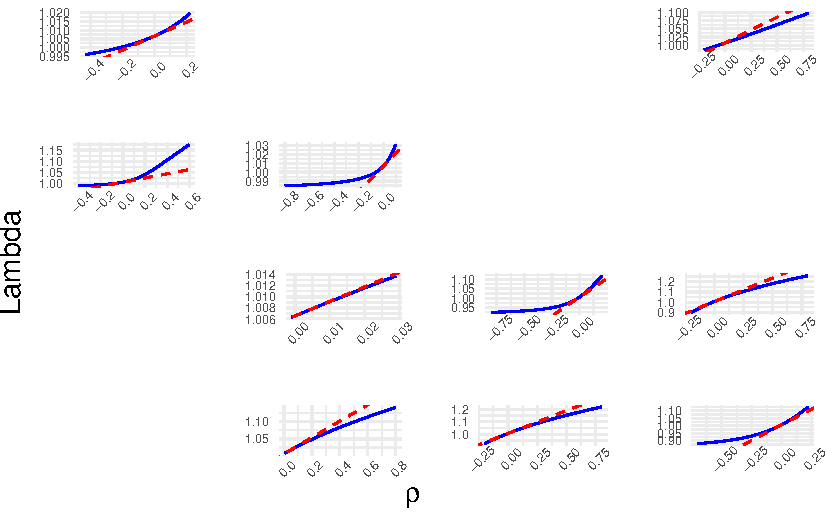
\includegraphics{113-Funciones_de_Transferencia_files/figure-pdf/unnamed-chunk-24-1.pdf}

Revisión:

RLT 2025-06-03

\begin{center}\rule{0.5\linewidth}{0.5pt}\end{center}

\phantomsection\label{refs}
\begin{CSLReferences}{1}{0}
\bibitem[\citeproctext]{ref-bialic2018using}
Bialic-Murphy L, Gaoue OG, Knight T. 2018. Using transfer function
analysis to develop biologically and economically efficient restoration
strategies. \emph{Scientific Reports} 8:2094.

\bibitem[\citeproctext]{ref-bierzychudek1999looking}
Bierzychudek P. 1999. Looking backwards: Assessing the projections of a
transition matrix model. \emph{Ecological Applications} 9:1278--1287.

\bibitem[\citeproctext]{ref-caswell2000matrix}
Caswell H. 1989. \emph{Matrix {P}opulation {M}odels}. Sinauer
Sunderland, MA.

\bibitem[\citeproctext]{ref-de2000elasticities}
De Kroon H, Van Groenendael J, Ehrlén J. 2000. Elasticities: A review of
methods and model limitations. \emph{Ecology} 81:607--618.

\bibitem[\citeproctext]{ref-ezard2010matrix}
Ezard TH, Bullock JM, Dalgleish HJ, Millon A, Pelletier F, Ozgul A,
Koons DN. 2010. Matrix models for a changeable world: The importance of
transient dynamics in population management. \emph{Journal of Applied
Ecology} 47:515--523.

\bibitem[\citeproctext]{ref-hastings2001transient}
Hastings A. 2001. Transient dynamics and persistence of ecological
systems. \emph{Ecology Letters} 4:215--220.

\bibitem[\citeproctext]{ref-hodgson2004methodological}
Hodgson DJ, Townley S. 2004. Methodological insight: Linking management
changes to population dynamic responses: The transfer function of a
projection matrix perturbation. \emph{Journal of Applied Ecology}
41:1155--1161.

\bibitem[\citeproctext]{ref-koons2007population}
Koons DN, Holmes RR, Grand JB. 2007. Population inertia and its
sensitivity to changes in vital rates and population structure.
\emph{Ecology} 88:2857--2867.

\bibitem[\citeproctext]{ref-stott2016perturbation}
Stott I. 2016. Perturbation analysis of transient population dynamics
using matrix projection models. \emph{Methods in Ecology and Evolution}
7:666--678.

\bibitem[\citeproctext]{ref-stott2012popdemo}
Stott I, Hodgson DJ, Townley S. 2012b. {p}opdemo: An {R} package for
population demography using projection matrix analysis. \emph{Methods in
Ecology and Evolution} 3:797--802.

\bibitem[\citeproctext]{ref-stott2012beyond}
Stott I, Hodgson DJ, Townley S. 2012a. Beyond sensitivity: Nonlinear
perturbation analysis of transient dynamics. \emph{Methods in Ecology
and Evolution} 3:673--684.

\bibitem[\citeproctext]{ref-stott2011framework}
Stott I, Townley S, Hodgson DJ. 2011. A framework for studying transient
dynamics of population projection matrix models. \emph{Ecology Letters}
14:959--970.

\bibitem[\citeproctext]{ref-tremblay2015stable}
Tremblay R, Raventos J, Ackerman J. 2015. When stable-stage equilibrium
is unlikely: Integrating transient population dynamics improves
asymptotic methods. \emph{Annals of Botany} 116:381--390. DOI:
\href{https://doi.org/10.1093/aob/mcv031}{10.1093/aob/mcv031}.

\end{CSLReferences}


\backmatter


\end{document}
